% !TeX program = xelatex
% Oracle Atlas working paper. Use XeLaTeX for the checked line layout; no shell escape required.
%%% Hugging Face: https://huggingface.co/organizations/Oracle4CEG
%%% Github Template: https://github.com/Oracle4CEG/Oracle4SD-Template
%%% GitHub: https://github.com/Oracle4CEG/Oracle4SD-Atlas/tree/main
\documentclass[11pt,a4paper]{article}
\usepackage{styles/preprint}

\hypersetup{
  pdftitle={A cross-protocol dataset of blockchain oracle incentives and accountability},
  pdfauthor={Huaiyu Jia, Siguang Li, Lin William Cong, Luyao Zhang},
  pdfsubject={Blockchain oracles, economic incentives, accountability, data provenance}
}

\begin{document}
\begin{center}
  {\LARGE\bfseries A cross-protocol dataset of blockchain\\oracle incentives and accountability\par}
  \vspace{0.9em}
  {\normalsize
    Huaiyu Jia\textsuperscript{a}\hspace{1.45em}
    Siguang Li\textsuperscript{a}\hspace{1.45em}
    Lin William Cong\textsuperscript{b}\hspace{1.45em}
    Luyao Zhang\textsuperscript{c,\hyperlink{correspondence-note}{*}}\par}
  \vspace{0.55em}
  {\small
    \textsuperscript{a} The Hong Kong University of Science and Technology (Guangzhou), Guangzhou, China\par
    \textsuperscript{b} Nanyang Technological University, Singapore\par
    \textsuperscript{c} Duke Kunshan University, Kunshan, China\par}
  \vspace{0.55em}
  {\footnotesize\itshape Working paper \enspace\textbullet\enspace October 2026\par}
\end{center}
\begingroup
\renewcommand{\thefootnote}{\fnsymbol{footnote}}
\footnotetext[1]{\hypertarget{correspondence-note}{}Corresponding author: Luyao Zhang. Duke Kunshan University, 8 Duke Avenue,\\ Kunshan, Suzhou, Jiangsu 215316, China. Email: \href{mailto:lz183@duke.edu}{lz183@duke.edu}.}
\endgroup
\setcounter{footnote}{0}
\vspace{-0.25em}
\begin{abstract}
Blockchain oracles connect smart contracts to external information, but their records use different units and accounting conventions. We present a data resource covering eight oracle branches, with five detailed panels and three narrower extensions. Native observations are linked to protocol rules and reconstructed lifecycles, distinguishing configured incentives, accruals, entitlements, payments and applied losses. UTC annotations preserve event times, epoch intervals and snapshots separately. Two derived products provide daily measurements within documented coverage and a request-level UMA prediction task with candidate inputs, availability records and protocol-resolution labels. Validation examines native identities, economic classifications, settlement accounting and a cross-chain dispute. The resulting resource supports descriptive research on participation, rewards and accountability while retaining differences in mechanism, asset and observation unit. Missing evidence remains explicit, and protocol adjudication is distinguished from independent verification of external facts.
\end{abstract}

\section{Introduction}

Blockchain oracles supply smart contracts with information that the ledger cannot observe. Prices and event outcomes enter contract execution through reporting, verification and dispute resolution~\cite{zhang2016towncrier,eskandari2021sok}. Participants may earn rewards, post capital, challenge reports or incur penalties. These arrangements determine both the information a contract accepts and the incentives for providing it~\cite{cong2019blockchain,cong2025oracleprimer}.

Public transactions do not make these incentives directly measurable. A transfer may combine returned principal with a reward; a negative accounting adjustment may precede any reduction in stake. Disputed requests can traverse several contracts or chains, whose versions, identifiers and accounting rules differ. Treating gross payouts as profit or accruals as realized losses changes the economic quantity being measured. Comparison requires lifecycle reconstruction under the applicable protocol rules.

Oracle mechanisms expose different aspects of economic accountability: proposals and adjudication, staking operations, reward epochs, signed updates or withdrawals. Oracle4SD Atlas selects branches for this variation and the historical evidence available to reconstruct it. The sample supports comparisons of specified activities; it is neither a census of oracle services nor a probability sample of the ecosystem.

The resource covers eight branches: five detailed panels for UMA, Chainlink, Tellor, Flare FTSOv2 and Pyth, and three narrower extensions for Chronicle, RedStone Push and DIA. The common accountability representation contains 105,588,120 typed observations, complemented by 22,723,389 economic components and 19,275,854 records meeting protocol-specific realization criteria. These representations overlap and use different observation units, so their counts cannot be added. Native records accompany the common fields, linking comparative measures to their supporting evidence.

The contribution is a measurement framework that connects protocol rules and native records to observable economic states. By distinguishing configured incentives, accrued adjustments, claimable entitlements, realized payments and applied losses, the resource supports descriptive research on participation, incentives and accountability within documented coverage boundaries. Figure~\ref{fig:ecosystem_scope} situates the sampled implementations within the wider oracle ecosystem, while Table~\ref{tab:protocol_sources} summarizes the scope of each branch. Comparisons remain conditional on observation units, historical rules and evidence availability. Protocol acceptance and financial execution are therefore interpreted separately from independent verification of external facts.

\begin{figure}[!htbp]
\centering
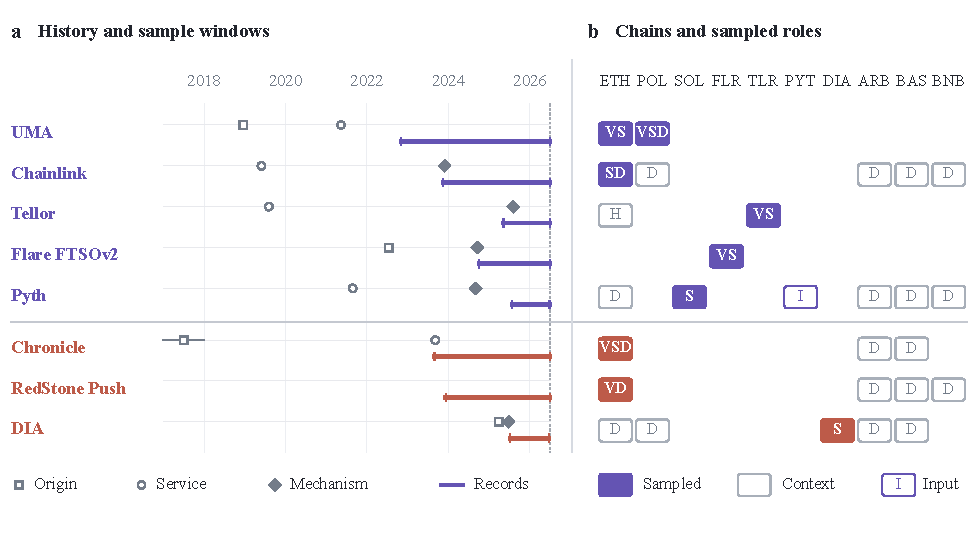
\includegraphics[width=\linewidth]{figures/ecosystem_scope.pdf}
\caption{Historical context and sampled scope of Oracle4SD Atlas. Purple denotes five detailed panels; coral denotes three narrower extensions. (a) Symbols mark project or network origins, service openings, and mechanism announcements or access milestones. Coloured segments delimit retained timestamps in one selected table per branch; they do not imply uninterrupted acquisition. The dashed line marks the 30 June 2026 cutoff. (b) Filled cells identify sampled chain roles; grey outlines show selected ecosystem context. V, verification/adjudication; S, economic settlement/accounting; D, delivery; H, historical implementation; I, retained derived inputs. ETH, Ethereum; POL, Polygon; SOL, Solana; FLR, Flare; TLR, tellor-1; PYT, Pythnet; DIA, Lasernet; ARB, Arbitrum; BAS, Base; BNB, BNB Chain. Dates and source evidence are provided in Appendix~\ref{app:scope}.}
\label{fig:ecosystem_scope}
\end{figure}


\section{Related work}

Research on oracles and research on blockchain datasets approach the same infrastructure from complementary directions. Oracle studies examine how external information is authenticated, aggregated and incentivized; data-resource studies establish reusable representations of transactions, entities and contracts. The present work connects these perspectives by making the relationship between native protocol evidence and economic measurement explicit. Tables~\ref{tab:oracle_related_work} and~\ref{tab:blockchain_datasets} summarize representative contributions without treating their differing units or purposes as directly comparable measures of scale.

\subsection{Oracle design, security and economic institutions}

Town Crier authenticates external data delivery through trusted hardware; DECO proves properties of data obtained over TLS~\cite{zhang2016towncrier,zhang2020deco}. The oracle systematization of knowledge reviews trust assumptions, attacks and mitigations~\cite{eskandari2021sok}. Adaptive conformal consensus provides conditional guarantees for aggregating reports, while SMARTCAT detects contracts associated with price-manipulation attacks~\cite{park2023acon,zhang2025smartcat}. These studies address information security; we reconstruct participant incentives and economic outcomes.

Empirical oracle studies provide a second foundation. A first look at DeFi oracles measures deployed price-oracle behavior, while Demystifying Pythia examines Chainlink usage, pricing and service quality on Ethereum~\cite{liu2021firstlook,kaleem2021pythia}. Economic research complements these observations by analyzing incentives, staking, decentralization and the integration of oracle networks with financial markets~\cite{cong2025oracleprimer,cong2026integration}. Together, these studies motivate an empirical representation that follows the economic process across participation, challenge, adjudication and settlement. The framework developed here retains those stages where the source evidence supports them, rather than assuming that every mechanism exposes an equivalent lifecycle.

The mechanisms represented in the Atlas expose different empirical objects. UMA and Tellor provide settings for studying contestable reporting, challenge participation and adjudicated outcomes~\cite{uma2026,tellorDisputes2026}. Chainlink's staking and feed records distinguish economic participation from observable service updates~\cite{chainlinkstaking2026}, while Flare FTSOv2 separates reward entitlements, provider conditions and subsequent claims~\cite{flareFTSO2026}. Pyth's OIS records connect publisher-related incentive states with staking operations and economic transfers within the retained historical window~\cite{pythOIS2026}. The narrower Chronicle, RedStone Push and DIA extensions add observations of challenge mechanisms, signed update delivery and staking withdrawals, respectively~\cite{chronicleDocs2026,redstoneDocs2026,diaDocs2026}. These branches contribute different parts of the measurement problem; their native records are not interchangeable observations of a universal oracle process.

Oracle economics and empirical studies motivate questions about incentives, monitoring, participation and service provision~\cite{cong2025oracleprimer,liu2021firstlook,kaleem2021pythia,cong2026integration}. The Atlas connects these questions to observation units, historical rules and economic stages. Documentation describes intended mechanisms; execution records show observed behavior. Signatures, consensus outcomes and payments do not independently establish external truth, and links to mechanism design do not establish theoretical equilibrium or security guarantees.

\begin{table}[!htbp]
\centering\tabstyle[atlaslight]
\caption{Oracle research and the measurement problem addressed here. ``Conceptual'' denotes a mechanism or taxonomy rather than a deposited cross-protocol economic panel. Contributions are compared as stated.}
\label{tab:oracle_related_work}
\begin{tabularx}{\linewidth}{@{}L{0.18\linewidth} L{0.21\linewidth} L{0.22\linewidth} Y@{}}
\toprule\tablehead
\thcell{document}{Study} & \thcell{compare}{Evidence focus} & \thcell{data}{Representation} & \thcell{coin}{Economic coverage} \\
\midrule
Town Crier~\cite{zhang2016towncrier} & Authenticated delivery & Trusted-hardware oracle architecture & External-data delivery; no cross-protocol economic lifecycle panel. \\
DECO~\cite{zhang2020deco} & Web-data provenance & Cryptographic proofs for TLS data & Data provenance and privacy; no reconstruction of oracle compensation or losses. \\
Oracle SoK~\cite{eskandari2021sok} & Security and trust & Taxonomy of designs, attacks and assumptions & Conceptual treatment of economic security and manipulation. \\
DeFi oracle measurement~\cite{liu2021firstlook} & Deployed price oracles & Reported values, deviations and operation & Selected operational measurements rather than harmonized incentive states. \\
Demystifying Pythia~\cite{kaleem2021pythia} & Chainlink on Ethereum & Usage, pricing and service quality & System-specific economic and usage measurements. \\
Oracle economics primer~\cite{cong2025oracleprimer} & Incentives and institutions & Economic framework for oracle mechanisms & Conceptual analysis of staking, decentralization and tokenomics. \\
\rowcolor{atlaslight}
\textbf{This resource} & Participation and accountability & Native lifecycles with typed economic components & Five detailed panels and three extensions; realized economics only where observable. \\
\bottomrule
\end{tabularx}
\end{table}


\subsection{Reusable blockchain data resources}

Elliptic represents Bitcoin transactions for illicit-activity classification, while Elliptic2 labels subgraphs of entity clusters~\cite{weber2019elliptic,bellei2024elliptic2}. Chartalist provides datasets for UTXO- and account-based blockchains; temporal Bitcoin datasets support entity and transaction graph analysis~\cite{shamsi2022chartalist,coquide2025orbitaal,schnoering2025bitcoin}. EX-Graph connects Ethereum and X, and Graphs of Graphs preserves relationships within and across token networks~\cite{wang2024exgraph,luo2024multichain}. Oracle research also requires the economic meaning of each request, report, entitlement and balance change.

Other resources link NFT and memecoin markets to network and visual features~\cite{nadini2021mapping,long2025coinmeme} or organize fine-grained DeFi events for forecasting~\cite{jia2026eventaware}. DIVE separates pre- and post-deployment contract representations for vulnerability analysis~\cite{alsunaidi2026dive}. We likewise retain multiple representations of an object, but interpret oracle participation and financial accountability through protocol-specific accounting rules.

\begin{table}[!htbp]
\centering\tabstyle[datasettint]
\caption{Representative blockchain datasets and analytical units. Counts refer to different objects and cannot be compared as sample sizes. Oracle4SD Atlas complements these resources with protocol-specific economic stages.}
\label{tab:blockchain_datasets}
\begin{tabularx}{\linewidth}{@{}L{0.16\linewidth} L{0.22\linewidth} L{0.24\linewidth} Y@{}}
\toprule\tablehead
\thcell{document}{Resource} & \thcell{data}{Observation unit} & \thcell{data}{Published scope} & \thcell{compare}{Analytical purpose} \\
\midrule
Elliptic~\cite{weber2019elliptic} & Bitcoin transaction & 203,769 nodes; 234,355 directed edges & Illicit-transaction classification and financial forensics. \\
Elliptic2~\cite{bellei2024elliptic2} & Entity cluster and labeled subgraph & 49.3 million clusters; 196.2 million edges; 121,810 labeled subgraphs & Money-laundering patterns at subgraph level. \\
Chartalist~\cite{shamsi2022chartalist} & Dataset-specific graph, address or transaction & Multiple UTXO- and account-based blockchain datasets & Reusable data access, graph construction and machine-learning benchmarks. \\
DIVE~\cite{alsunaidi2026dive} & Ethereum smart contract & 22,330 contracts; pre- and post-deployment representations & Vulnerability analysis with lifecycle-specific features. \\
\rowcolor{datasettint}
\textbf{This resource} & Typed protocol-native observation & 105,588,120 harmonized observations; eight branches & Incentive and accountability measurement, with native units and economic realization states retained. \\
\bottomrule
\end{tabularx}
\end{table}


Comparative oracle research needs shared concepts tied to native roles, timing and economic states. Our layered representations distinguish announced incentives from claimable entitlements, transfers from participant gain, and institutional decisions from external truth. Validation preserves these distinctions.

\section{Methods}

Construction links protocol evidence to economic interpretation before defining common analytical fields. Figure~\ref{fig:oracle_dgp} summarizes source registration, native decoding, lifecycle reconstruction and harmonization. Unresolved identities, open lifecycles and unobservable outcomes remain explicit. The common schema supports comparison while preserving protocol-specific meanings.

\begin{figure}[!htbp]
\centering
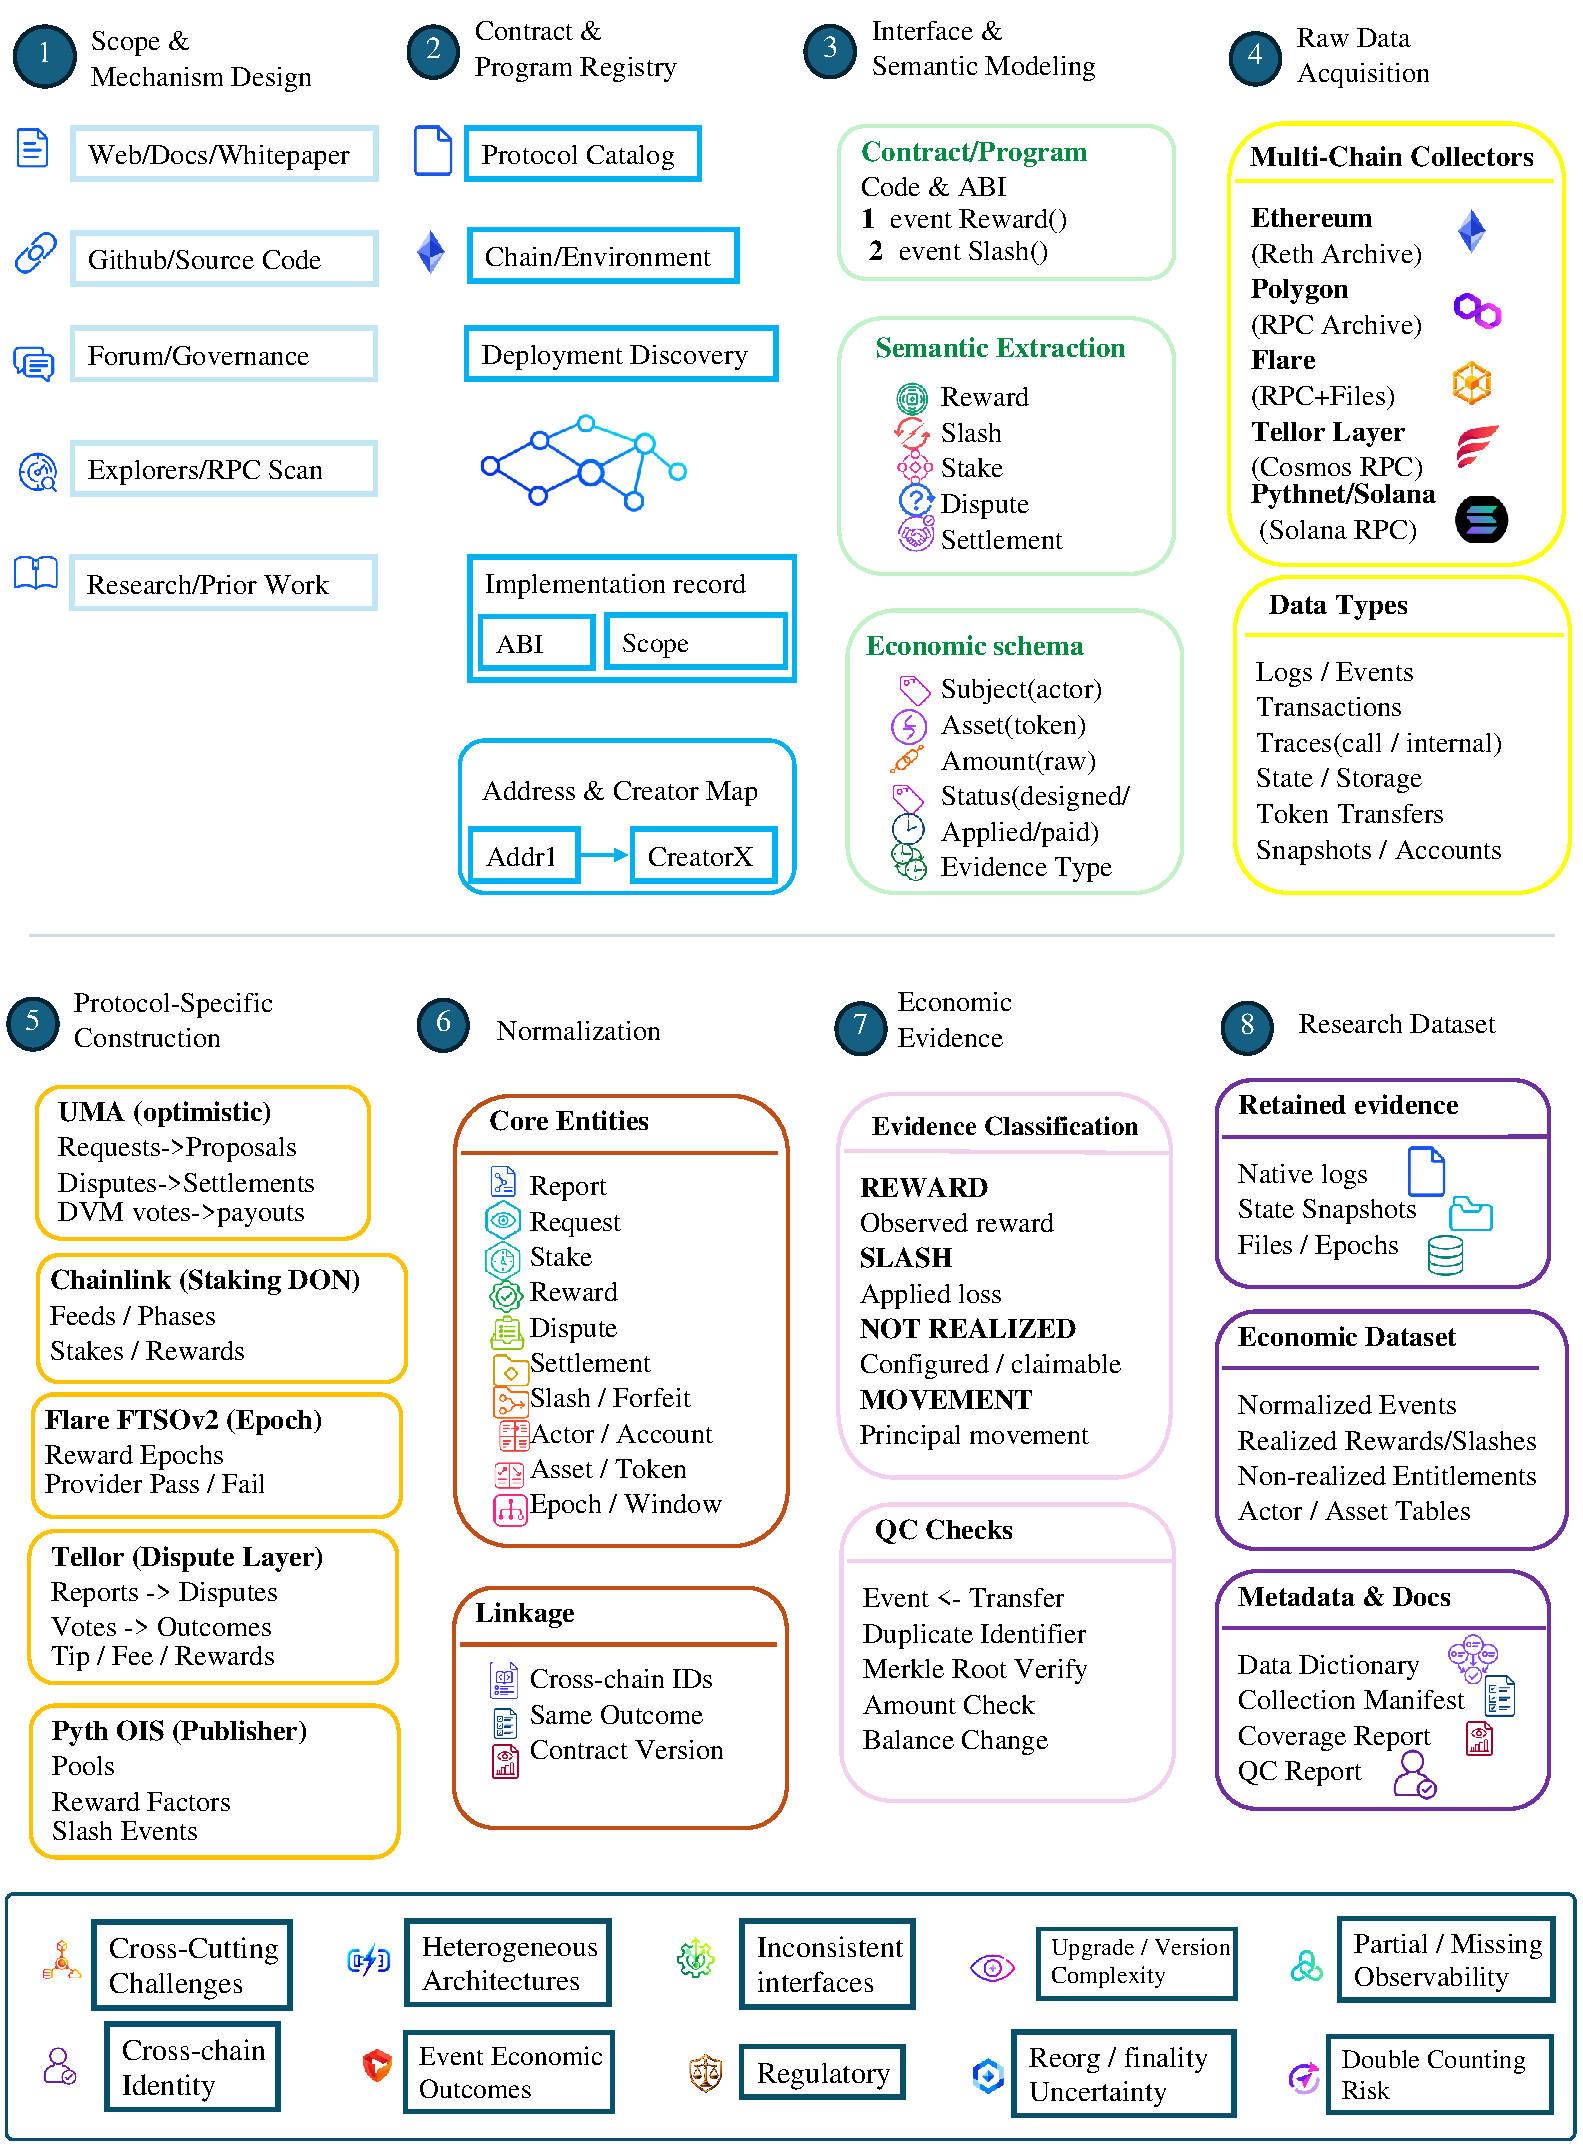
\includegraphics[width=0.99\linewidth]{figures/overview_restored.pdf}
\caption{Construction and validation workflow. Stages 1--4 register sources, define native semantics and acquire evidence; stages 5--8 reconstruct supported lifecycles and economic states for analysis and documentation. The lower strip lists measurement challenges. Checks require evidence; protocol decisions do not establish external truth.}
\label{fig:oracle_dgp}
\end{figure}

\subsection{Scope, selection and historical boundaries}

The discovery registry contains 56 oracle or related mechanism categories and 366 protocol--oracle relationships. It supports source discovery and ecosystem description, not probability sampling. Eight branches are selected for their economic mechanisms, identifiable historical records and scope for reconstruction. Each branch denotes a specified mechanism and implementation, including the chain roles observed in its records.

UMA, Chainlink, Tellor, Flare FTSOv2 and Pyth provide five detailed native panels. Chronicle, RedStone Push and DIA add narrower observations of challenge, update delivery and staking activities. Panel breadth implies neither complete histories nor equivalent variables or protocol quality. Only registered versions and services are included. Table~\ref{tab:protocol_sources} summarizes branch scope; Appendix~\ref{app:scope} lists sources and exclusions.

Chain roles are distinguished by function. A verification or adjudication chain records the relevant acceptance or dispute-resolution process; an economic settlement chain records the associated payment or applied balance change; and a delivery chain records provision of the oracle output to a consuming application. A single network may serve several roles. In the linked UMA disputes studied here, Polygon hosts the OOv2 lifecycle and observed local settlement flows, whereas Ethereum hosts VotingV2 adjudication. Linking these records establishes a relationship between protocol objects and does not, by itself, establish a cross-chain token transfer. The eight branches consequently do not denote eight independent blockchains.

The common upper observation cutoff is 30 June 2026 at 23:59:59 UTC. Table-level temporal support is documented separately from protocol history in Appendix~\ref{app:temporal}. The temporal register identifies deployment-bound scans, implementation changes, retained-history limits and cohort restrictions without treating a first event as a deployment date. Lower boundaries vary with deployment, implementation changes, historical source availability and collection limits. Project founding dates, production-service launches, deployment boundaries, scanned intervals and first observed events are distinct quantities. An interval between the first and last retained events does not establish uninterrupted observation. Transaction histories and retained state panels may also have different temporal support, as in the Pyth OIS branch. Historical interpretation requires an implementation applicable to the observation; unresolved source bindings and acquisition gaps remain limitations. Current protocol documentation supplies architectural context~\cite{uma2026,chainlinkstaking2026,tellorDisputes2026,flareFTSO2026,pythOIS2026,chronicleDocs2026,redstoneDocs2026,diaDocs2026}, while Appendix~\ref{app:scope} distinguishes that context from retained historical evidence.

\begin{table}[!htbp]
\centering\tabstyle[registrytint]
\caption{Measurement roles, implementation scope and historical boundaries of the eight oracle branches. Coverage refers to registered sources, not all services of a protocol. The upper cutoff is 30 June 2026, 23:59:59 UTC. Appendix~\ref{app:scope} separates deployment, scanning and retained-event boundaries.}
\label{tab:protocol_sources}
\begin{tabularx}{\linewidth}{@{}L{0.105\linewidth} L{0.22\linewidth} L{0.255\linewidth} Y@{}}
\toprule\tablehead
\textbf{Branch} & \textbf{Implementation and chain} & \textbf{Registered coverage} & \textbf{Measurement role and main exclusion} \\
\midrule
UMA & Ethereum VotingV2; Polygon OOv2 and adapters & DVM blocks 16,697,232--25,433,938; Polygon contract-specific starts through 89,439,336 & Proposals, disputes, adjudication and settlement. Other UMA versions and deployments are outside the registered scope. \\
Chainlink & Ethereum Staking v0.2; ETH/USD proxy and feed phases & Staking from block 18,572,190; registered sources through 25,433,938 & Staking economics and selected feed updates. Other feeds, networks and services are excluded. \\
Tellor & \texttt{tellor-1} modules, ABCI events and block results & Heights 1--19,890,860; first report at height 317 & Reports, disputes, votes, payments and restrictions. Legacy Ethereum Tellor is excluded. \\
Flare FTSOv2 & Flare RewardManager, VoterRegistry and reward artifacts & Closed reward epochs 228--410; cutoff block 64,054,789 & Entitlements, provider conditions and claims. Table coverage differs; aggregate claims may resist attribution. \\
Pyth & Solana OIS transactions and retained Pythnet-derived inputs & Transaction archive from 11 September 2024; 49 retained closed state epochs & Publisher--epoch states, staking and transfers. State coverage is shorter; other products and delivery networks are excluded. \\
\midrule
Chronicle & Registered Ethereum validator and challenge contracts & Registered log scan 0--25,433,938; deployment dates are separate & Reports, challenges and challenge rewards. Rewards are not a complete publisher-compensation ledger. \\
RedStone Push & Registered Ethereum Push adapters and feeds & Registered log scan 0--25,433,938; deployment dates are separate & Signed publication and Push updates. Other delivery modes and full AVS economics are excluded. \\
DIA & Registered Lasernet staking contracts & Deployment block 3,874,186 through cutoff 31,302,665 & Withdrawals, returned principal and rewards. This is not a complete price-production or delivery audit. \\
\bottomrule
\end{tabularx}
\end{table}


\subsection{Source acquisition and native decoding}

For each branch, a source register identifies the network, contract or program, implementation, collection interval and retrieval interface. EVM-compatible branches use historical logs, supplemented where necessary by transactions, receipts, block metadata and token-transfer evidence. ERC-20 transfers are retained when they help separate principal, fees and rewards from a settlement event. Tellor instead combines tellor-1 module state, ABCI events and block results; multiple reports within one block produce a one-to-many expansion into 82,866,640 report observations. Pyth evidence is located by Solana transaction signatures and outer or inner instruction positions. Flare combines on-chain records with official reward-calculation artifacts, preserving the distinction between entitlement and claim.

Decoding follows the registered version and cutoff. Polygon UMA has 626,578 raw records, including five unknown event topics retained only in the raw collection. Chainlink staking has 175,015 collected logs, yielding 174,890 decoded events and 125 unclassified records. Unclassified records do not indicate absent economic behavior. Tables retain native keys, integer amounts, asset identifiers and decimal precision.

\subsection{Lifecycle reconstruction and cross-chain linkage}

Decoded records are joined where the native mechanism identifies a relationship between successive states. UMA requests link proposals, disputes, DVM adjudication and settlement through reconstructed request identifiers. For requester $r$, identifier $i$, timestamp $t$ and ancillary data $a$, the identifier is
\begin{equation}
 q = \operatorname{Keccak256}\!\left(\operatorname{pack}(r,i,t,a)\right),
 \label{eq:requestid}
\end{equation}
where $\operatorname{pack}$ denotes the protocol's packed ABI encoding. The reconstructed OOV2 panel contains 42,676 request rounds: 41,826 settle by the cutoff and 850 remain open. Other mechanisms require different objects. For example, 46,723 retained Chainlink ETH/USD answer updates define 46,722 adjacent service windows, and 13 Tellor jail events are paired with 13 release events to reconstruct reporter restrictions.

Cross-chain identity is established through version-aware ancillary-data transformations and native request construction. A UMA link receives Grade A only when the registered bridge or adapter rule identifies one unique DVM request. Of 835 attempted links, 832 meet this deterministic definition and three remain unmatched. The grade describes the identity of a reconstructed object; it does not certify the factual correctness of the oracle's decision. Retaining unmatched and unfinished objects prevents the apparent completeness of an analytical table from replacing evidence about the underlying process. The worked case links request, proposal, dispute, DVM resolution and Polygon settlement. Each endpoint is located by its chain, transaction and log position. The retained evidence supports the object linkage and elapsed intervals; intermediate relay operations are represented separately where their transactions are not retained.

\subsection{Economic states and settlement accounting}

An economic observation is classified by its state and evidentiary basis. Table~\ref{tab:economic_states} distinguishes configured incentives, accrued rewards or penalties, claimable entitlements, realized payments, applied losses, principal, refunds and fees. The distinctions are protocol-specific. UMA challenge status requires native challenge evidence, and settlement is not inferred merely from a transfer-like event. Tellor SUPPORT outcomes refer to acceptance of the challenge and rejection of the challenged report. Negative DVM accruals remain distinct from an observed reduction in staked principal. Pyth reward rates are not token reward amounts, and Flare participation restrictions are not automatically monetary losses.

UMA settlement provides a concrete accounting example. Let $B$ be the effective bond, $F$ the final fee and $R$ the configured reward, all measured in the smallest integer unit of the same asset. Posted principal is $P=B+F$. For disputed requests, the identifiable winner component is $W=B-\lfloor B/2\rfloor$, while the protocol component is $F_{\mathrm{protocol}}=\lfloor B/2\rfloor+F$. Expected gross payouts follow the registered contract and adapter rules:
\begin{align}
 G_{\mathrm{undisputed}} &= B+F+R, \nonumber\\
 G_{\mathrm{disputed}} &= B+F+W+R_{\mathrm{settlement}}.
 \label{eq:payout}
\end{align}
Here $R_{\mathrm{settlement}}$ is the reward attributable to settlement under the applicable adapter; refunds and rollovers are not automatically participant income. Exact integer reconciliation requires $\Delta_{\mathrm{payout}}=G_{\mathrm{actual}}-G_{\mathrm{expected}}=0$.

In Section~\ref{sec:case}, a 1,000-unit payout comprises 750 in principal and 250 in gain before costs. A configured five-unit reward is refunded or rolled over as observed. Net profit requires cost data. UMA settlements are checked against token movements, Chainlink separates transfer-requiring events from accounting adjustments, and Flare reconciliation retains only components supported by the claim evidence.

\begin{table}[!htbp]
\centering\tabstyle[economictint]
\caption{Economic states distinguished in reconstruction. Each classification requires the evidence specified by the originating protocol. A lifecycle need not expose every state.}
\label{tab:economic_states}
\begin{tabularx}{\linewidth}{@{}L{0.20\linewidth} L{0.33\linewidth} Y@{}}
\toprule\tablehead
\thcell{clock}{State} & \thcell{coin}{Economic meaning} & \thcell{compare}{Interpretation rule} \\
\midrule
Configured incentive & Reward specified in protocol parameters & A design parameter; not automatically participant income. \\
Accrued reward or penalty & Calculated entitlement or liability & Distinct from subsequent payment or application; counting both may duplicate one change. \\
Claimable entitlement & Amount eligible for a claim & An unclaimed entitlement is not a zero payment or a realized transfer. \\
Paid reward & Observed transfer or realized protocol credit & Realized only when qualifying cash-flow or state evidence is present. \\
Applied slash & Reduction applied to a participant's balance or principal & Requires observed application, beyond a penalty calculation or accrual. \\
Principal deposit or return & Capital posted and subsequently recovered & Kept separate from rewards and fees; returned capital is not profit. \\
Refund or rollover & Incentive returned or carried to another state & Not attributed to the current participant without supporting evidence. \\
Protocol fee & Amount charged or retained under protocol rules & Separated from participant reward and principal. \\
\bottomrule
\end{tabularx}
\end{table}


\subsection{Harmonization, missingness and documentation}

Common fields retain protocol, unit, role, actor or beneficiary, lifecycle identity, time, asset, economic stage, source and evidence status. The accountability layer contains 105,588,120 typed observations; the economic layer contains 22,723,389 components, including 19,275,854 meeting branch-specific payment or applied-state criteria. These overlapping layers describe the same underlying processes at different levels.

Timestamp availability differs from coverage: a valid clock on every retained row does not prove complete collection, and a missing clock does not imply an absent event. Epoch and snapshot clocks remain distinct from canonical event time. Missing values can indicate inapplicability, unexposed quantities, incomplete collection, decoding problems or unfinished lifecycles. They are not automatically zero. Where supported, schemas distinguish complete, partial, verified-zero, unknown, unavailable and not-applicable coverage; right censoring is recorded separately. Deduplication uses native keys and preserves legitimate multiplicity across representations and economic components. Table~\ref{tab:processing_pipeline} summarizes these operations.

\begin{table}[!htbp]
\centering\tabstyle[acquisitiontint]
\caption{Processing operations and their outputs. Rows describe transformations rather than statistically independent populations: operations may expand, aggregate, join or decompose their inputs.}
\label{tab:processing_pipeline}
\begin{tabularx}{\linewidth}{@{}L{0.21\linewidth} L{0.39\linewidth} Y@{}}
\toprule\tablehead
\thcell{clock}{Operation} & \thcell{document}{Input and rule} & \thcell{data}{Output} \\
\midrule
Source registration & Network, contract or program, historical version, interval and interface & Branch-specific collection specification. \\
Acquisition and qualification & Logs, transactions, receipts, block or module state, signatures and protocol artifacts; cutoff and decoding rules & Qualified source records, with unresolved decoding outcomes retained. \\
Native decoding & Protocol event and state definitions; integer amounts and native keys & Protocol-native tables. \\
Lifecycle reconstruction & Request, dispute, claim, epoch or other native object relationships & Supported lifecycle objects and open cases. \\
Cross-chain linkage & Version-specific identifier and ancillary-data transformations & Deterministic matches, link grades and unmatched cases. \\
Economic-state mapping & Native lifecycle and accounting evidence & Configured, accrued, claimable, paid, applied, returned, refunded and fee components. \\
Funds-flow reconciliation & Expected quantities against observed transfers or applied state changes & Realization flags and accounting differences. \\
Harmonization & Shared concepts with native units and source links retained & 105,588,120 typed accountability observations. \\
Realization filtering & Protocol-specific evidence conditions applied to 22,723,389 economic components & 19,275,854 qualifying realized components. \\
Documentation & Dictionaries, schemas, coverage information, source registers and validation results & Interpretable data and reconstruction materials. \\
\bottomrule
\end{tabularx}
\end{table}


Documentation records native identifiers, source registers, input inventories, schemas, variable definitions and validation rules. Quality controls assess selected key relationships, lifecycle orderings, cutoff conditions, economic identities and deterministic links. The accompanying artifacts identify the tested populations and the evidence available for reconstruction. Their traceability supports inspection of specific mappings, while leaving incomplete historical acquisition and unresolved source ancestry visible.

\subsection{Temporal harmonization}
\label{sec:temporal}

Native timestamps are expressed in UTC while retaining their original values and precision. Each time field is documented by its source, unit and role in the protocol. The field \codefield{event_time_utc} identifies when an event was recorded or executed. Request-reference timestamps, oracle payload times and scheduled deadlines are represented separately because they can refer to a different point in the lifecycle. Records sharing a timestamp retain their native block, transaction, log or instruction order.

Unix-second and millisecond values are converted without rounding. Textual timestamps are interpreted using their recorded timezone; timezone-naive values are treated as UTC where this convention is established by the source. Missing EVM event times are recovered only when another retained record identifies the timestamp of the same block on the same chain. Conflicting matches are rejected and unmatched observations remain undated. The provenance of recovered timestamps is recorded with the data.

Epoch observations retain their start and end times as half-open intervals $[a_e,b_e)$. Payment, snapshot and retrieval times describe separate events and are stored independently. In particular, an epoch-end label does not establish when a reward became claimable or was paid. Historical state recovered from a later snapshot also requires care when assessing information available at a past decision time.

Daily windows begin at midnight UTC, and weekly windows run from Monday to the following Monday. Epoch totals remain attached to their native support intervals. Daily aggregation therefore requires an event-level measure or an explicit allocation rule, together with evidence that the relevant period was observed. Appendix~\ref{app:temporal} describes the native clocks and temporal limitations of each branch.


\subsection{UMA prediction-task construction}
\label{sec:prediction}

The prediction task asks whether UMA's eventual resolution differs from the proposed price. Each observation is one request, and the decision time $T_0$ is the proposal event. For proposed price $p_i$ and resolved price $z_i$, the label is $Y_i=\mathbf{1}\{z_i\ne p_i\}$. Native values are compared as integers. Indeterminate and early-expiration values retain their own classes; neither is recoded as a binary answer.

Eligibility requires a challenged request, a unique deterministic DVM link, consistent resolution values and a reconciled settlement transfer. Because selection is retrospective, the task concerns adjudication among selected disputes, not challenge risk for new requests. Challenge, resolution and settlement fields supply outcome evidence and are excluded from predictive inputs.

The sixteen candidate features describe incentives, timing, ancillary-data length, participant history and adapter identity. Proposer and requester histories are calculated separately from requests settled before the current proposal in native execution order. Rates are missing without prior settlements. Proposal latency begins at the request event; liveness ends at expiry. Parameter-derived features require evidence of availability at $T_0$ and carry a separate status. Appendix~\ref{app:prediction} defines the features and their information boundary.

\subsection{Daily economic measurements}
\label{sec:daily}

Daily observations use midnight-to-midnight UTC intervals and retain branch, implementation, actor role, asset, unit and economic stage. Feasibility distinguishes derivable measures, additional acquisition requirements, inapplicable quantities and unresolved cases. Appendix~\ref{app:daily} defines aggregation and denominators.

Payments enter the daily product only under the relevant realization rule. UMA rewards are separated from returned principal and forfeited bonds. VotingV2 net stake applications retain their own economic stage and are not added to request-level accruals; Tellor withdrawals into stake and Pyth transfers to stake custody retain those destinations. Flare fee burns are excluded from participant payments. Chainlink claims require a matched transfer and an execution timestamp. An unobserved day is left unfilled, and totals over retained records are not presented as complete protocol totals.

Participation measures count addresses within a named role. Reward concentration is calculated among recipients with positive observed payments, separately by asset and economic stage. For completed UMA requests, delay runs from the request event to settlement, and escrow exposure integrates observed balances between successive transfers. Only unambiguous closed request flows with nonnegative intermediate balances are included; the measure includes funded rewards while held and does not represent unresolved capital obligations. Flare signing weights and thresholds are retained on their native epoch intervals; they are not interpreted as daily payments or token collateral.

\section{Data records}

Ten logical products cover eight protocol branches, the UMA prediction task and daily measurements. Each may contain several linked tables. Common representations support comparison; native tables preserve mechanism-specific timing and accounting. Table~\ref{tab:files} lists the principal components, with types, definitions and relationships documented in the catalogue and dictionaries.

\begin{table}[!htbp]
\centering\tabstyle
\caption{Data organization. Tables may contribute to several representations; row counts are not additive.}
\label{tab:files}
\begin{tabularx}{\linewidth}{@{}L{.25\linewidth}L{.21\linewidth}Y@{}}
\toprule Component & Form & Contents \\ \midrule
Eight native branches & Parquet and retained source artifacts & Requests, reports, votes, claims, transfers, policies and state observations. \\
Common representations & Typed Parquet projections & Shared accountability fields and economic components with native source references. \\
Temporal annotations & UTC fields and dictionaries & Event times, reference clocks, epochs, snapshots and missing-time status. \\
UMA prediction task & Request and availability tables & Protocol-resolution label, sixteen candidate features and retrospective selection rules. \\
Daily measurements & Daily and epoch companion tables & Typed counts and amounts, recipient aggregates, completed-request delays, capital exposure and policy weights. \\
Supporting evidence & Ledger and case tables & Old/new semantic values, source locators, case intervals and cashflows. \\
Metadata and reproduction & Catalogues, dictionaries and code & Ten logical products, physical recordsets, fingerprints and executable examples. \\
\bottomrule
\end{tabularx}
\end{table}


\subsection{Native records and table relationships}

Native tables preserve the object meaningful to the originating protocol. The UMA OOV2 panel contains 42,676 request lifecycles, while the Tellor micro-report table contains 82,866,640 reports. Other examples include 18,468,735 Flare claim events and 518,560 decoded Pyth OIS instructions. These quantities count requests, reports, claims and instructions, respectively. A comparison that treats them as equivalent oracle events would confuse differences in data granularity with differences in institutional activity. Within a branch, related evidence can also be stored separately: UMA request-level lifecycle and payout fields link to token-flow records rather than repeating each transfer inside the request table.

Identifiers follow the strongest available native structure. EVM logs use chain, transaction and log position; Tellor relies on module-specific report metadata; Solana evidence uses signatures and instruction positions. Table~\ref{tab:record_keys} summarizes these keys and their relationships. Checks on the named UMA, Chainlink and cross-chain linkage tables assess selected primary-key and foreign-key constraints. A one-to-many relationship can represent several events within a lifecycle or several components within one settlement. It is therefore a relationship to interpret, rather than a duplication to remove automatically.

\begin{table}[!htbp]
\centering\tabstyle[normalizationtint]
\caption{Native units, identifier construction and logical relationships. One-to-many relationships describe scientific objects, not mandatory duplication in every physical table. Native ordering is authoritative; physical row order is not.}
\label{tab:record_keys}
\begin{tabularx}{\linewidth}{@{}L{0.18\linewidth} L{0.32\linewidth} Y@{}}
\toprule\tablehead
\thcell{data}{Unit} & \thcell{link}{Identifier} & \thcell{clock}{Relationship and interpretation} \\
\midrule
EVM log & Chain, transaction hash and log index & A transaction can contain several logs. Order by block and log position; retain receipt and block evidence. \\
UMA OOV2 request & \codefield{oo_request_id}; requester, identifier, timestamp and ancillary data & One request links several lifecycle events and transfers. Request, proposal, dispute and settlement times remain distinct. \\
UMA DVM request or voter record & \codefield{dvm_request_id}; voter and source-event location for actor-level records & One request can link many voters and adjustments. Accrual and applied stake change are different observations. \\
Tellor report & \codefield{query_id}, reporter and \codefield{meta_id}; block-position namespace for the common key & Multiple reports can contribute to an aggregate. Native module metadata replaces a universal EVM transaction/log key. \\
Flare entitlement or claim & Epoch, beneficiary and claim type; transaction/log position for a claim & Entitlements and claims are not universally one-to-one. Epoch end differs from claim time. \\
Pyth instruction or transfer & Signature and \codefield{outer_instruction_index}; inner position for token transfers & One transaction can contain several instructions and transfers. Reconstruct time from block time and instruction positions. \\
Common observation & \codefield{accountability_event_id}, protocol namespace, \codefield{native_table} and \codefield{accountability_unit_id} & Native-to-common mapping can be one-to-many. The retained native unit defines the statistical object. \\
Economic component & \codefield{evidence_id} and originating table/event identity & One settlement can yield several components. \codefield{do_not_sum_group} identifies related components at risk of double counting. \\
\bottomrule
\end{tabularx}
\end{table}


\subsection{Common accountability and economic representations}

The common accountability table contains 105,588,120 rows and 50 columns. Each row projects a native observation while retaining protocol, unit, role, source and evidence status. Requests, reports, disputes, epochs, staking observations and service windows remain distinct units. Cross-protocol aggregation must therefore retain protocol, native table, unit type and unit identity to establish comparability.

Economic components are represented in a separate 22,723,389-row, 28-column table. Its fields record the mechanism, stage, actor, counterparty, amount, asset, source object, evidence class and validation status. A stricter 19,275,854-row representation uses the same physical schema but requires qualifying evidence of payment or an applied economic change. It overlaps the broader component table and is not an independent sample. Stage, actor, asset and the documented grouping of related components must be considered together: adding an accrued penalty to a later applied slash can count the same economic process twice.

\subsection{Dictionaries, types and interpretive states}

Documentation operates at two levels. The conceptual dictionary defines 33 economic variables: 28 core measures and five supporting variables. The core measures comprise four participation or concentration variables, nine incentive or friction variables, and fifteen outcome or accountability variables. Supporting entries identify the episode, decision time, challenge deadline, cross-chain link grade and provenance. Their definitions specify units, derivation, decision-time availability, evidence class, missingness and validation rules. The physical dictionary describes the columns in each table, including the derived products and their supporting evidence. Conceptual variables and physical columns serve different purposes; the catalogue records their relationships rather than treating their counts as alternative estimates of dataset dimensionality.

Table~\ref{tab:dictionary} summarizes selected field families. Raw monetary amounts are stored as integer-valued strings and interpreted with their asset and decimal fields, avoiding loss from floating-point conversion. The common representation includes integer Unix-second labels. Separate UTC annotations preserve native timestamp precision and distinguish event times from epoch boundaries and snapshots. JSON schemas define required fields and controlled values, including the 85-field cross-chain observation schema. Where supported, coverage distinguishes complete, partial, verified-zero, unknown, unavailable and not-applicable conditions; right censoring separately identifies unfinished lifecycles. Schema checks establish consistency with these tested definitions, rather than proving every historical interpretation correct.

\begin{table}[!htbp]
\centering\tabstyle[semantictint]
\caption{Selected field families. Dictionaries define the schema; amounts require asset and decimal fields.}
\label{tab:dictionary}
\begin{tabularx}{\linewidth}{@{}L{0.19\linewidth} L{0.35\linewidth} Y@{}}
\toprule\tablehead
\thcell{document}{Field family} & \thcell{data}{Representative fields} & \thcell{compare}{Type and analytical meaning} \\
\midrule
Identity and mechanism & \codefield{oracle_network}, \codefield{mechanism_family}, \codefield{native_table}, \codefield{security_chain}, \codefield{delivery_chain} & Strings identifying the mechanism, native table and chain context. \\
Observation unit & \codefield{accountability_unit_type}, \codefield{accountability_unit_id}, \codefield{event_granularity} & Strings or controlled values defining what a row represents. \\
Time & \codefield{event_time_unix}, \codefield{reward_accrual_time_unix}, \codefield{reward_payment_time_unix} & Integer-second labels in the common representation; separate UTC annotations distinguish event, epoch, payment and snapshot times (Appendix~\ref{app:temporal}). \\
Actors and roles & \codefield{actor}, \codefield{actor_role}, \codefield{counterparty}, \codefield{counterparty_role} & Native addresses or identifiers and interpreted roles; not natural-person identities. \\
Reward & \codefield{reward_class}, \codefield{reward_amount_raw}, \codefield{reward_asset}, \codefield{reward_asset_decimals} & Integer string, asset identity and decimal precision. Economic stage determines interpretation. \\
Penalty and forfeiture & \codefield{penalty_accrued_raw}, \codefield{principal_slashed_raw}, \codefield{bond_forfeited_raw}, \codefield{fee_forfeited_raw}, \codefield{reward_forfeited_raw} & Integer strings with asset metadata; distinguishes accrual, applied principal loss and other forfeitures. \\
Principal & \codefield{principal_locked_raw}, \codefield{principal_returned_raw}, \codefield{principal_asset} & Integer strings and asset metadata; separates exposed or recovered capital from gain. \\
Outcome basis & \codefield{truth_basis}, \codefield{outcome_status}, \codefield{external_truth_available} & Strings and booleans describing the basis for an outcome; protocol resolution is not external ground truth. \\
Source and rule & \codefield{source_event}, \codefield{source_tx}, \codefield{source_block}, \codefield{source_contract}, \codefield{rule_id}, \codefield{parameter_version} & Strings and integers linking observations to native evidence and the interpretation rule. \\
Realization & \codefield{economic_kind}, \codefield{economic_evidence_class}, \codefield{realization_status}, \codefield{amount_raw}, \codefield{signed_amount_raw}, \codefield{cashflow_verified}, \codefield{state_delta_verified} & Controlled values, integer strings and booleans recording the economic stage and evidence for realization. \\
\bottomrule
\end{tabularx}
\end{table}


Curated tables use Zstandard-compressed Apache Parquet; metadata use UTF-8 CSV or JSON, and source packages use JSONL or compressed JSONL. The revised catalogue distinguishes the earlier deposit's 95 tables and application artifacts from the new task, daily measurements and evidence ledgers. Registers, inventories and validation identify acquisition evidence, reconstruction inputs and outputs.

\subsection{Temporal metadata}

Native tables retain the original timestamps and identifiers alongside UTC fields for the clocks supported by each source. The common accountability and economic representations use companion tables joined by their retained record identifiers. These companions distinguish execution times, epoch boundaries and missing clocks without altering the original observations. Their definitions specify temporal meaning, precision and the reason a time is unavailable. Analyses using the common representations should use these supported UTC clocks; the earlier integer-second labels remain for provenance.

Temporal metadata record each table's available interval and missing timestamps. Execution times, epoch intervals, deadlines and snapshots retain distinct meanings, allowing comparable periods to be selected without treating every timestamp as an instantaneous event.

\subsection{Derived products and supporting evidence}

The UMA task contains one row per eligible request, a sixteen-field feature dictionary and a feature-level availability record. The daily product contains typed measurements, recipient-level payment aggregates, completion delays and observed escrow exposure, together with a separate historical Flare signing-policy table. The latter retains epoch support because signing weights are defined by the policy interval.

The correction ledger records old and revised field values for identifiable native objects. The cross-chain case retains the event register, elapsed intervals, cashflow components and unresolved evidence links. These supporting tables document how the measurements were obtained; their rows are not additional independent oracle observations. Appendix~\ref{app:products} describes the ten products and their relationships.

\section{Data overview}

Figure~\ref{fig:daily} illustrates the temporal support and units of selected measurements. Daily participation and payments are available for different retained populations, while UMA delay describes completed requests and Flare concentration describes epoch-specific signing policies. These quantities are interpreted within their branch, role and observation window. Open requests remain in the lifecycle records, days without eligible retained events remain unfilled, and policy weights are kept separate from token amounts. The broader feasibility assessment in Appendix~\ref{app:daily} identifies which comparisons require additional evidence.
\begin{figure}[!htbp]
\centering
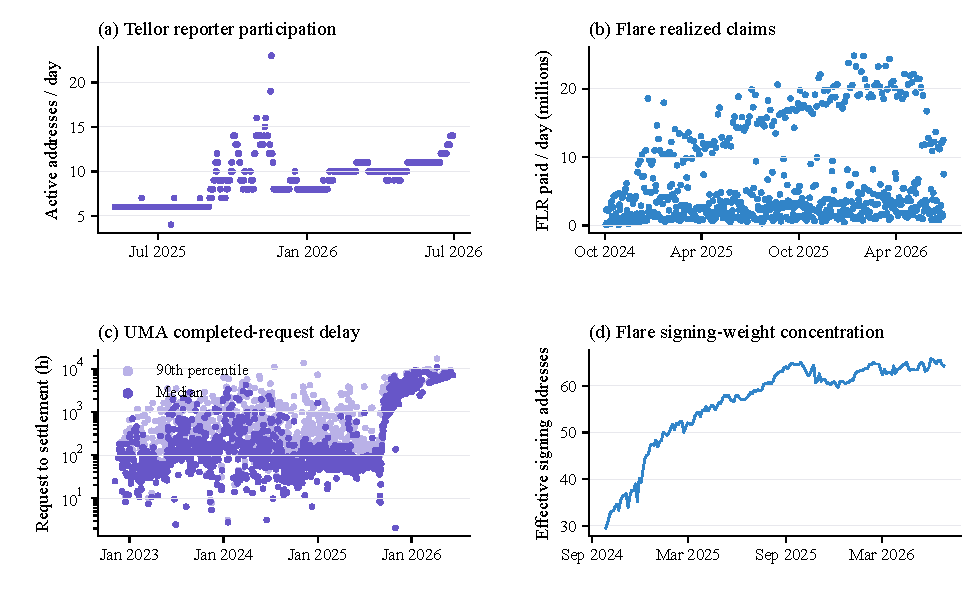
\includegraphics[width=0.99\linewidth]{figures/daily_gallery.pdf}
\caption{Selected measurements from the daily product and its epoch-level companion. (a) Distinct Tellor reporter addresses with retained reports on each observed day. (b) Flare claims in FLR, excluding fee burns. (c) Median and 90th-percentile request-to-settlement delay among flow-reconciled UMA USDC.e requests completed on that day; the vertical axis is logarithmic. (d) Effective signing-address count, $1/\sum_i w_i^2$, using normalized Flare signing-policy weights within each retained epoch. Address counts do not identify independent entities.}
\label{fig:daily}
\end{figure}

\section{Technical validation}

Validation tests structural, economic and computational properties within specified populations. Readable files, unique identifiers, balanced settlements and reproducible calculations establish different properties; none alone proves complete acquisition or external truth. We distinguish documented checks, direct table checks, historical protocol validation and replay from retained inputs.

\subsection{Structural consistency and economic semantics}

Structural checks examine source identities, native keys, table relationships and lifecycle order. Request-level records and voter-level accounting entries are tested separately because their units differ. Cross-chain checks test whether linked records identify the same protocol object.

Economic classification is checked against the historical implementation, the recorded execution and the financial quantity being measured. For each correction, an object-level record preserves the previous value, the revised value, the source locator and the applied rule. Source binding is strongest for the retained VotingV2 implementation; the OOv2 and Tellor bindings remain qualified, as described in Appendix~\ref{app:semantics}.

Table~\ref{tab:semantic_repair} reports classification errors and corrections for UMA challenges and settlements, Tellor outcomes and DVM penalty accruals. Corrected UMA winner-reward components total 201,500 USDC.e and 1,250 USDC, kept separate by asset. These reclassify existing settlements rather than add payments. Of thirteen Tellor disputes, three support the challenge and have positive applied slashes; ten reject it and have no positive applied slash under the recorded checks. SUPPORT denotes a decision for the disputer.

\begin{table}[!htbp]
\centering\tabstyle
\caption{Economic-semantic checks and correction evidence. Native populations may overlap across rules.}
\label{tab:semantic_repair}
\begin{tabularx}{\linewidth}{@{}L{.19\linewidth}Yrr@{}}
\toprule
Rule & Evidence and interpretation & Population & Before / after \\
\midrule
UMA challenge & Dispute event and nonzero disputer; a proposal alone is insufficient. & 42,676 & 40,992 / 0 \\
UMA settlement & Settled lifecycle and matched token movement. Open requests remain unsettled. & 42,676 & 850 / 0 \\
UMA winner gain & Contract payout rule and settlement transfer; returned principal is separate. & 42,676 & 834 / 0 \\
Tellor outcome & SUPPORT accepts the challenge and rejects the report. & 13 & 13 / 0 \\
Tellor applied loss & Final dispute outcome; initiation escrow is distinct from applied loss. & 13 & 10 / 0 \\
DVM accrual & Signed request accrual; an applied stake change requires separate evidence. & 2,663,684 & 947,128 / 0 \\
\bottomrule
\end{tabularx}
\end{table}


\begin{figure}[!htbp]
\centering
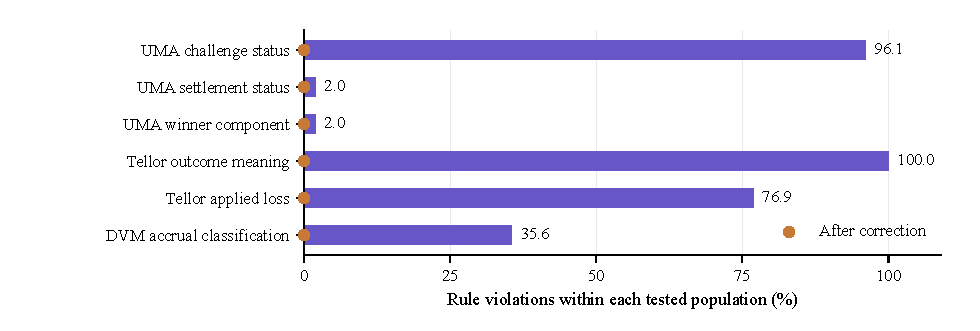
\includegraphics[width=0.99\linewidth]{figures/semantic_gallery.pdf}
\caption{Economic-semantic corrections within six separately defined populations. Bars show the proportion violating each rule before correction; orange markers show the corresponding proportion after applying the rule. Populations and rule evidence are specified in Table~\ref{tab:semantic_repair}. A request may be affected by more than one rule.}
\label{fig:semantic}
\end{figure}


In the DVM population, 947,128 negative accruals had been classified as applied principal losses without evidence of a corresponding reduction. Reclassifying them as penalty accruals preserves the accounting state without asserting realized loss. Valid records still require interpretation under the mechanism's rules.

\subsection{Accounting reconciliation and object identity}

All 41,826 settled UMA requests satisfy the recorded integer payout identity,
\begin{equation}
 \Delta_{\mathrm{payout}}=G_{\mathrm{actual}}-G_{\mathrm{expected}}=0,
 \label{eq:payoutcheck}
\end{equation}
with the associated transfer-matching checks passing under the applicable contract and adapter rules. Chainlink checks identify 51,372 qualified staking and reward records: 50,772 require transfers and match the recorded token movements, while 600 are accounting-only adjustments. The historical Flare report documents Merkle-root and claim reconciliation for 183 closed reward epochs. Those retained results are distinguished from a fresh rerun of the complete chain-level validation.

Of 835 UMA cross-chain link attempts, 832 meet the deterministic Grade-A rule and three remain unmatched. Pyth replay checks reward-state calculations over 49 retained closed epochs. These results support tested links and accounting; completeness, row ancestry and external truth remain unverified.

\subsection{Computational reproducibility}

A worked UMA case links archived events to a request lifecycle and reconciles economic records with token movements. Repeated executions check consistency for identical inputs and code.

These evaluations concern reconstruction from retained evidence. Reacquiring historical data also depends on archive access, interface behaviour and the original collection boundaries. The acquisition records document those conditions separately from the computational checks.

\subsection{Temporal consistency}

Temporal checks compare UTC conversions with native values and verify observation order. Millisecond clocks preserve fractional seconds. Native and UTC selections agree for the tested daily and weekly windows. Epoch checks verify retained boundaries and the assignment of observations at interval endpoints.

Missing timestamps are assessed separately from event absence. Exact block matching improves temporal availability for some EVM records, while unresolved observations retain a missing-time status. Appendix~\ref{app:temporal} summarizes these limitations and the distinction between timestamp availability and historical coverage.


\subsection{Daily aggregation and prediction-task checks}

Daily validation checks that grouped event counts and integer monetary totals agree with their eligible native inputs. Escrow exposure is checked by comparing daily balance-duration totals with the integral over the request's observed transfer intervals. A valid timestamp is required for assignment to a day; eligible observations without one remain in the source population and in the missing-time accounting.

The prediction-task checks examine request uniqueness, cohort membership, target construction and feature timing. Role-history counts and rates are compared with a separate direct selection of prior settlements. The checks also preserve the distinction between a native event observed by the proposal and a historical parameter whose availability requires additional source binding. Feature distributions and missingness are provided in Appendix~\ref{app:prediction} to support inspection of the task data.

\subsection{Worked cross-chain settlement}
\label{sec:case}

The worked dispute links four Polygon transactions to an Ethereum VotingV2 resolution. Polygon records the request, proposal, challenge and local settlement. Checks verify receipt status, blocks, event positions and request identity. Figure~\ref{fig:case} presents timing and cashflows; Appendix~\ref{app:case} lists events and relay gaps.

Proposal occurs about 7.7 hours after the request, followed shortly by a challenge. DVM resolution follows about 92.2 hours later, and Polygon settlement follows after roughly 22 minutes. These endpoints cannot separate transport, scheduling and adjudication. Early expiration retains its nonbinary meaning.

Each party posts 750 USDC.e. The winner receives 1,000 USDC.e: 750 in returned principal and 250 in gain. The fee recipient receives 500. The configured reward is refunded or rolled over separately. Flows balance, but net profit requires costs. Cross-chain identity does not establish a bridge transfer.
\begin{figure}[!htbp]
\centering
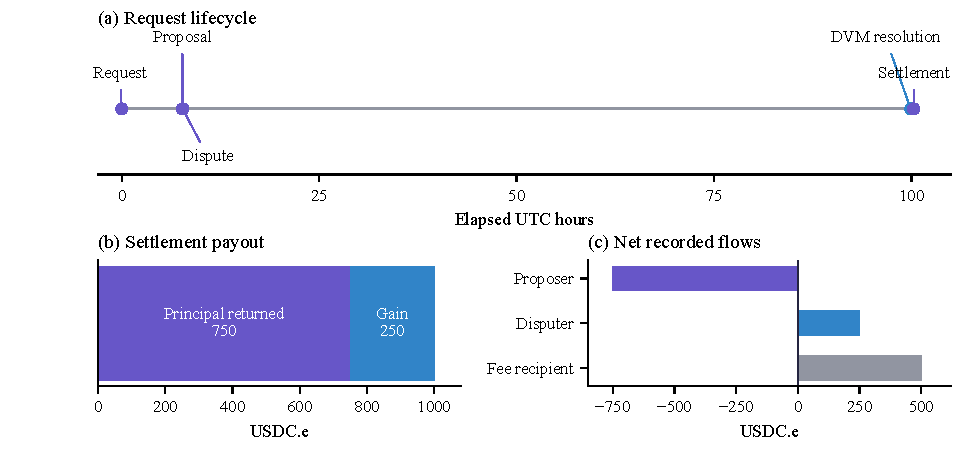
\includegraphics[width=0.99\linewidth]{figures/cross_chain_gallery.pdf}
\caption{A linked UMA dispute. (a) Events on a proportional elapsed-time axis: Polygon events are purple and the Ethereum resolution is blue. The proposal and challenge are close in time. The interval between challenge and resolution includes unobserved intermediate transport steps. (b) The winner's gross payout separates principal from gain. (c) Participant and fee-recipient net flows balance in USDC.e, before additional costs.}
\label{fig:case}
\end{figure}

\section{Research use and interpretation}

Research use should begin with a mechanism-specific question and an explicitly defined observation unit. Table~\ref{tab:research_opportunities} connects the eight branches to research questions, available observations and additional evidence requirements. These mappings identify opportunities for reuse rather than report tests of the proposed hypotheses. Analyses should retain implementation version, actor role, asset, economic stage and observation window, and establish comparability for the particular measure being studied. A shared schema facilitates this work but does not, by itself, identify causal effects or make different native activities interchangeable.

\begin{table}[!htbp]
\centering\tabstyle[registrytint]
\caption{Research opportunities supported by the eight branches. Rows identify potential uses and evidence needed for stronger claims; they are not findings or tests of mechanism-design guarantees.}
\label{tab:research_opportunities}
\begin{tabularx}{\linewidth}{@{}L{0.13\linewidth} L{0.25\linewidth} L{0.26\linewidth} Y@{}}
\toprule\tablehead
\textbf{Branch / literature} & \textbf{Question} & \textbf{Available observations} & \textbf{Further evidence needed} \\
\midrule
UMA~\cite{cong2025oracleprimer,uma2026} & How do challenges and settlement timing vary with incentive commitments? & Bonds, configured rewards, liveness and request lifecycles. & Monitoring opportunities, costs, factual labels and an identification design for incentive effects. \\
Chainlink~\cite{liu2021firstlook,kaleem2021pythia,chainlinkstaking2026} & How do participation and reward realization relate to service provision? & Stake operations, reward claims and selected ETH/USD updates. & Node--service mappings, historical obligations and external references. \\
Tellor~\cite{cong2025oracleprimer,tellorDisputes2026} & How is accountability executed in observed disputes? & Reports, disputes, votes, payments and restrictions. & Broader comparable disputes, challenge opportunities and independent factual outcomes. \\
Flare FTSOv2 \mbox{\cite{cong2025oracleprimer,flareFTSO2026}} & How are reward entitlements formed and realized? & Provider conditions, entitlements, claims and epoch signing policies. & Eligibility--claim matching; historical runtime binding and entity-level ownership for control analysis; external prices for accuracy. \\
Pyth~\cite{cong2025oracleprimer,pythOIS2026} & How do participation and economic realization vary across OIS regimes? & Retained publisher--epoch states, staking instructions and transfers. & Effective rule-change times, comparable windows and treatment of concurrent changes. \\
Chronicle~\cite{eskandari2021sok,chronicleDocs2026} & Which reporting and challenge pathways are observable? & Registered reports, challenges and challenge rewards. & Historical signer sets, thresholds and factual references; full compensation remains unobserved. \\
RedStone Push~\cite{eskandari2021sok,redstoneDocs2026} & How do signed publications translate into Push updates? & Publication and update records for registered adapters and feeds. & Historical update settings and external references; AVS economics requires separate acquisition. \\
DIA~\cite{cong2025oracleprimer,diaDocs2026} & How much of a withdrawal is capital recovery versus reward? & Staking withdrawals and principal/reward components. & Deposit--withdrawal matching and costs for position returns; feeder lineage for price-production analysis. \\
\bottomrule
\end{tabularx}
\end{table}


DuckDB, PyArrow and compatible tools can query Parquet tables through column selection and filtering. The repository notebook provides a smaller reconstruction example; the catalogue and dictionaries document table relationships and variables. Monetary values require asset and decimal fields. Event order follows native chronology, not row position. Addresses identify accounts, not their owners.

Economic aggregation must distinguish configured rewards, accruals, entitlements, payments and applied penalties. Returned principal differs from gain, and net profit requires costs. Check related components before summation; keep USDC.e and USDC separate unless a justified conversion rule applies. Missing, unavailable and inapplicable values are not zeros. Retain censored lifecycles as needed.

The UMA task supports modelling subject to retrospective selection and decision-time constraints. Causal analysis requires an identification strategy and further evidence.

Repositories provide data, code, documentation and an issue tracker. Reuse should record input versions and the computational environment, distinguish archived reconstruction from historical reacquisition, and preserve native meanings when extending analyses or reporting corrections.

\section{Data and code availability}

The data are available through the project's Hugging Face repository.\footnote{Data and documentation: \url{https://huggingface.co/datasets/Oracle4CEG/OracleEconLab-Oracle-Incentives-v1/tree/atlas-utc-20261029}.} The release contains eight protocol products, the UMA prediction task and daily measurements, together with source registers, evidence ledgers and validation materials. Its catalogue records table identities, variable definitions and relationships. Earlier experimental outputs remain archived separately from these ten products.

The processing repository provides reconstruction scripts, figure sources and a tutorial with bounded examples for all eight branches.\footnote{Processing code: \url{https://github.com/Oracle4CEG/Oracle4SD-Atlas/tree/71c0e19d3ae2b47d763243371f1bfb97750db61d}.} The tutorial includes an executed local notebook. Input versions and execution records distinguish archived reconstruction from fresh public-interface acquisition; independent-reader and Google-hosted execution remain pending. Appendix~\ref{app:reproduction} describes the reproducibility boundaries.


\FloatBarrier
% Bibliography audited against primary publications and publisher-deposited metadata.
\begin{thebibliography}{99}
\raggedright
\interlinepenalty=10000

\bibitem{zhang2016towncrier}
Zhang, F., Cecchetti, E., Croman, K., Juels, A. \& Shi, E.
\href{https://doi.org/10.1145/2976749.2978326}{Town Crier: An authenticated data feed for smart contracts.}
In \emph{Proceedings of the ACM SIGSAC Conference on Computer and Communications Security}, 270--282 (2016).
doi: \nolinkurl{10.1145/2976749.2978326}.

\bibitem{eskandari2021sok}
Eskandari, S., Salehi, M., Gu, W. C. \& Clark, J.
\href{https://doi.org/10.1145/3479722.3480994}{SoK: Oracles from the ground truth to market manipulation.}
In \emph{Proceedings of the 3rd ACM Conference on Advances in \linebreak Financial Technologies}, 127--141 (2021).
doi: \nolinkurl{10.1145/3479722.3480994}.

\bibitem{cong2019blockchain}
Cong, L. W. \& He, Z.
\href{https://doi.org/10.1093/rfs/hhz007}{Blockchain disruption and smart contracts.}
\linebreak
\emph{The Review of Financial Studies} \textbf{32}, 1754--1797 (2019).
doi: \nolinkurl{10.1093/rfs/hhz007}.

\bibitem{cong2025oracleprimer}
Cong, L. W., Fox, L., Li, S. \& Zhou, L.
\href{https://doi.org/10.1016/j.jcorpfin.2025.102800}{A primer on oracle economics.}
\emph{Journal of Corporate Finance} \textbf{94}, 102800 (2025).
doi: \nolinkurl{10.1016/j.jcorpfin.2025.102800}.

\bibitem{zhang2020deco}
Zhang, F., Maram, D., Malvai, H., Goldfeder, S. \& Juels, A.
\href{https://doi.org/10.1145/3372297.3417239}{DECO: Liberating web data using decentralized oracles for TLS.}
In \emph{Proceedings of the ACM SIGSAC Conference on Computer and Communications Security}, 1919--1938 (2020).
doi: \nolinkurl{10.1145/3372297.3417239}.

\bibitem{park2023acon}
Park, S., Bastani, O. \& Kim, T.
\href{https://www.usenix.org/conference/usenixsecurity23/presentation/park}{$\mathrm{ACon}^{2}$: Adaptive conformal consensus for provable blockchain oracles.}
In \emph{32nd USENIX Security Symposium}, 3313--3330 (2023).


\bibitem{zhang2025smartcat}
Zhang, B., He, N., Hu, X., Ma, K. \& Wang, H.
\href{https://www.usenix.org/conference/usenixsecurity25/presentation/zhang-bosi}{Following Devils' Footprint: Towards real-time detection of price manipulation attacks.}
In \emph{34th USENIX Security Symposium}, 4127--4145 (2025).


\bibitem{liu2021firstlook}
Liu, B., Szalachowski, P. \& Zhou, J.
\href{https://doi.org/10.1109/DAPPS52256.2021.00010}{A first look into DeFi oracles.}
\linebreak
In \emph{IEEE International Conference on Decentralized Applications and Infrastructures}, \linebreak 39--48 (2021).
doi: \nolinkurl{10.1109/DAPPS52256.2021.00010}.

\bibitem{kaleem2021pythia}
Kaleem, M. \& Shi, W.
\href{https://doi.org/10.1007/978-3-662-63958-0_10}{Demystifying Pythia: A survey of ChainLink oracles usage on Ethereum.}
In \emph{Financial Cryptography and Data Security: FC 2021 International \linebreak Workshops}, 115--123 (2021).
doi: \nolinkurl{10.1007/978-3-662-63958-0_10}.

\bibitem{cong2026integration}
Cong, L. W., Prasad, E. S. \& Rabetti, D.
\href{https://doi.org/10.2139/ssrn.4495514}{Financial and informational integration through oracle networks.}
Working paper (2023; revised March 2026).
doi: \nolinkurl{10.2139/ssrn.4495514}.

\bibitem{weber2019elliptic}
Weber, M., Domeniconi, G., Chen, J., Weidele, D. K. I., Bellei, C., Robinson, T. \& Leiserson, C. E.
\href{https://arxiv.org/abs/1908.02591}{Anti-money laundering in Bitcoin: Experimenting with graph convolutional networks for financial forensics.}
\emph{KDD Workshop on Anomaly Detection in Finance} (2019).


\bibitem{bellei2024elliptic2}
Bellei, C., Xu, M., Phillips, R., Robinson, T., Weber, M., Kaler, T., Leiserson, C. E., Arvind \& Chen, J.
\href{https://arxiv.org/abs/2404.19109}{The shape of money laundering: Subgraph representation learning on the blockchain with the Elliptic2 dataset.}
\emph{KDD Workshop on Machine Learning in Finance} (2024).


\bibitem{shamsi2022chartalist}
Shamsi, K., Victor, F., Kantarcioglu, M., Gel, Y. \& Akcora, C. G.
\href{https://doi.org/10.52202/068431-2531}{Chartalist: Labeled graph datasets for UTXO and account-based blockchains.}
\emph{Advances in Neural Information \linebreak Processing Systems} \textbf{35} (2022).
doi: \nolinkurl{10.52202/068431-2531}.

\bibitem{coquide2025orbitaal}
Coquid\'e, C. \& Cazabet, R.
\href{https://doi.org/10.1038/s41597-025-04595-8}{A temporal graph dataset of Bitcoin entity--entity transactions.}
\emph{Scientific Data} \textbf{12}, 337 (2025).
doi: \nolinkurl{10.1038/s41597-025-04595-8}.

\bibitem{schnoering2025bitcoin}
Schnoering, H. \& Vazirgiannis, M.
\href{https://doi.org/10.1038/s41597-025-04684-8}{Bitcoin research with a transaction graph dataset.}
\emph{Scientific Data} \textbf{12}, 404 (2025).
doi: \nolinkurl{10.1038/s41597-025-04684-8}.

\bibitem{wang2024exgraph}
Wang, Q., Zhang, Z., Liu, Z., Lu, S., Luo, B. \& He, B.
\href{https://openreview.net/forum?id=juE0rWGCJW}{EX-Graph: A pioneering dataset bridging Ethereum and X.}
\emph{International Conference on Learning Representations} (2024).


\bibitem{luo2024multichain}
Luo, B., Zhang, Z., Wang, Q. \& He, B.
\href{https://doi.org/10.52202/079017-0894}{Multi-chain graphs of graphs: A new approach to analyzing blockchain datasets.}
\emph{Advances in Neural Information Processing \linebreak Systems} \textbf{37}, 28490--28514 (2024).
doi: \nolinkurl{10.52202/079017-0894}.

\bibitem{nadini2021mapping}
Nadini, M., Alessandretti, L., Di Giacinto, F., Martino, M., Aiello, L. M. \& Baronchelli, A.
\href{https://doi.org/10.1038/s41598-021-00053-8}{Mapping the NFT revolution: Market trends, trade networks, and visual features.}
\linebreak
\emph{Scientific Reports} \textbf{11}, 20902 (2021).
doi: \nolinkurl{10.1038/s41598-021-00053-8}.

\bibitem{long2025coinmeme}
Long, H.-W., Wong, N.-M. \& Cai, W.
\href{https://doi.org/10.1145/3701716.3715561}{Bridging culture and finance: A multimodal analysis of memecoins in the Web3 ecosystem.}
In \emph{Companion Proceedings of the ACM Web Conference}, 1158--1161 (2025).
doi: \nolinkurl{10.1145/3701716.3715561}.

\bibitem{jia2026eventaware}
Jia, H., You, J., Liu, J., Luo, Y. \& Sun, S.
\href{https://doi.org/10.1145/3770855.3817502}{Towards event-aware forecasting in DeFi: Insights from on-chain automated market maker protocols.}
In \emph{Proceedings of the 32nd ACM SIGKDD Conference on Knowledge Discovery and Data Mining V.2}, 9171--9182 (2026).
doi: \nolinkurl{10.1145/3770855.3817502}.

\bibitem{alsunaidi2026dive}
Alsunaidi, S. J., Aljamaan, H. \& Hammoudeh, M.
\href{https://doi.org/10.1038/s41597-026-07025-5}{DIVE: A multi-label smart contract vulnerability dataset.}
\emph{Scientific Data} \textbf{13}, 664 (2026).
doi: \nolinkurl{10.1038/s41597-026-07025-5}.

\bibitem{uma2026}
UMA.
\href{https://docs.uma.xyz/developers/optimistic-oracle}{Optimistic Oracle v2.}
(accessed 13 October 2026).

\bibitem{chainlinkstaking2026}
Chainlink.
\href{https://chain.link/economics/staking}{Chainlink staking.}
(accessed 13 October 2026).

\bibitem{tellorDisputes2026}
Tellor.
\href{https://docs.tellor.io/tellor/running-tellor/disputes-and-reporter-governance}{Disputes and reporter governance.}
(accessed 13 October 2026).

\bibitem{flareFTSO2026}
Flare Network.
\href{https://dev.flare.network/ftso/scaling/overview}{FTSOv2 scaling.}
(accessed 13 October 2026).

\bibitem{pythOIS2026}
Pyth Network.
\href{https://docs.pyth.network/oracle-integrity-staking/mathematical-representation}{Oracle Integrity Staking: Mathematical representation.}
(accessed 13 October 2026).

\bibitem{chronicleDocs2026}
Chronicle Labs.
\href{https://docs.chroniclelabs.org/}{Chronicle documentation.}
(accessed 13 October 2026).

\bibitem{redstoneDocs2026}
RedStone.
\href{https://docs.redstone.finance/}{RedStone documentation.}
(accessed 13 October 2026).

\bibitem{diaDocs2026}
DIA.
\href{https://www.diadata.org/docs/home}{DIA documentation.}
(accessed 13 October 2026).


\bibitem{atlasScopeMetadata2026}
Oracle4SD.
\href{https://github.com/Oracle4CEG/Oracle4SD-Atlas/tree/1dc0dfc3bc919e64f43a110bf29b75ef0e34459c/metadata}{Historical acquisition profiles, contract registry, source manifests and time-coverage metadata.}
Oracle4SD-Atlas, commit \texttt{1dc0dfc3bc919e64f43a110bf29b75ef0e34459c} (2026).


\bibitem{risklabsHistory2026}
Risk Labs.
\href{https://risklabs.foundation/}{Our story: UMA whitepaper publication.}
accessed 26 October 2026.


\bibitem{umaOOlaunch2021}
Lambur, H.
\href{https://medium.com/uma-project/introducing-umas-optimistic-oracle-d92ce5d1a4bc}{Introducing UMA's Optimistic Oracle.}
13 May 2021.


\bibitem{chainlinkMainnet2019}
Chainlink.
\href{https://chain.link/blog/chainlink-connected-consensus-on-ethereum}{Chainlink: Connected consensus on Ethereum.}
30 May 2019.


\bibitem{chainlinkV022023}
Chainlink.
\href{https://chain.link/blog/chainlink-staking-v0-2-now-live}{Chainlink Staking v0.2 is now live.}
28 November 2023.


\bibitem{tellorMainnet2019}
Tellor.
\href{https://tellor.io/tellor-launches-to-mainnet/}{Tellor launches to mainnet.}
5 August 2019.


\bibitem{tellorPublic2025}
Tellor.
\href{https://tellor.io/blog/layer-mainnet-open-to-public/}{Tellor Layer mainnet open to public.}
4 August 2025.


\bibitem{flareGenesis2025}
Flare Network.
\href{https://flare.network/news/flare-third-anniversary}{Flare at three: Powering a connected and data-rich DeFi ecosystem.}
14 July 2025.


\bibitem{flareV22024}
Flare Network.
\href{https://flare.network/news/ftsov2-more-data-delivered-faster}{FTSOv2: More data, delivered faster.}
16 September 2024.


\bibitem{pythMainnet2021}
Pyth Network.
\href{https://www.pyth.network/blog/pyth-network-mainnet}{Pyth Network mainnet launch.}
26 August 2021.


\bibitem{pythOISintro2024}
Pyth Network.
\href{https://www.pyth.network/blog/oracle-integrity-staking-incentivizing-safer-price-feeds-for-a-more-secure-defi}{Oracle Integrity Staking: Incentivizing \linebreak safer price feeds for a more secure DeFi.}
2 September 2024.


\bibitem{chroniclePublic2023}
Chronicle Protocol.
\href{https://www.globenewswire.com/en/news-release/2023/09/05/2737624/0/en/Chronicle-Protocol-the-Exclusive-5B-Oracle-of-MakerDAO-Opens-Access-to-All-Web3-Builders.html}{Chronicle Protocol opens access to all Web3 builders.}
5 September 2023.


\bibitem{diaStaking2025}
DIA.
\href{https://www.diadata.org/blog/post/mainnet-staking-blockchain-oracle-grants/}{DIA launches mainnet staking and blockchain oracle grants campaign.}
24 June 2025.


\bibitem{diaMainnet2025}
DIA.
\href{https://www.diadata.org/blog/post/dia-lumina-mainnet-live/}{Lasernet mainnet is live: DIA Lumina's full rollout is here.}
26 March 2025.


\end{thebibliography}


\clearpage
\appendix
\setcounter{table}{0}
\renewcommand{\thetable}{S\arabic{table}}
\renewcommand{\theHtable}{appendix.\arabic{table}}
\section{Scope and sources}
\label{app:scope}

\subsection{Selection and scope boundaries}
Branch selection combines a measurement question with identifiable historical evidence. UMA and Tellor cover contestable reporting and adjudication; Chainlink covers staking and selected feed service; Flare covers entitlements and claims; Pyth covers publisher--epoch incentives and staking. Chronicle, RedStone and DIA add narrower challenge, Push-update and withdrawal observations. Table~\ref{tab:protocol_sources} defines these boundaries. The registry is not exhaustive or probabilistic; exclusions apply only to this release.

Economic comparison requires an interpretable native unit, identifiable implementation and source. Monetary amounts also require an asset and accounting stage. Signed updates can describe delivery without measuring publisher payments; withdrawals can separate principal and reward without proving price accuracy. These limits govern the research opportunities in Table~\ref{tab:research_opportunities}.

\subsection{Historical implementations and source register}
\label{app:implementations}
Table~\ref{tab:implementation_register} records the principal contracts, programs and source versions. The accompanying source register describes their network roles, observation units, historical boundaries and inclusion criteria, including the Tellor modules and Chainlink feed proxy. Acquisition records preserve the connection between each sampled implementation and the evidence used to reconstruct it~\cite{atlasScopeMetadata2026}.

Deployment, scan and observation boundaries remain separate. Chronicle and RedStone searches begin at block 0, a search bound rather than a deployment block. Pyth's archive starts at a transaction timestamp rather than an EVM block. A pinned repository or cutoff runtime does not prove an unchanged historical implementation. Deployment times and implementation intervals require supporting metadata.

\begingroup
\small\setlength{\tabcolsep}{4pt}\renewcommand{\arraystretch}{1.12}
\begin{longtable}{@{}L{0.12\linewidth} L{0.40\linewidth} L{0.42\linewidth}@{}}
\caption{Historical implementation and source register. Declared deployment blocks and retained source versions reproduce the deposited metadata; they are not newly verified deployment or runtime histories. Full addresses, source commits and unresolved fields are preserved in the accompanying files.}\label{tab:implementation_register}\\
\toprule
\textbf{Branch} & \textbf{Principal identifier and chain role} & \textbf{Retained source, boundary and limitation} \\
\midrule\endfirsthead
\multicolumn{3}{l}{\small\itshape Table \thetable\ continued}\\
\toprule
\textbf{Branch} & \textbf{Principal identifier and chain role} & \textbf{Retained source, boundary and limitation} \\
\midrule\endhead
\midrule\multicolumn{3}{r}{\small\itshape Continued on next page}\\\endfoot
\bottomrule\endlastfoot
\textbf{UMA} & Polygon (137), OOv2: \path{0xee3afe347d5c74317041e2618c49534daf887c24}. Ethereum (1), VotingV2: \path{0x004395edb43efca9885cedad51ec9faf93bd34ac}. Registered adapters and tunnels are listed separately in the contract CSV. Roles: verification, settlement and delivery, by implementation. & Retained UMA source \texttt{a16ee53125c4} and adapter source \texttt{8b76cc9e0d46}. Declared OOv2 deployment: Polygon block 29,786,052; earliest registered adapter: 23,569,780; cutoff: 89,439,336. DVM: 16,697,232--25,433,938. Historical runtime intervals are not fully established by cutoff code hashes. \\ \addlinespace[3pt]
\textbf{Chainlink} & Ethereum (1), community pool: \path{0xbc10f2e862ed4502144c7d632a3459f49dfcdb5e}; operator pool: \path{0xa1d76a7ca72128541e9fcacafbda3a92ef94fdc5}; ETH/USD proxy: \path{0x5f4ec3df9cbd43714fe2740f5e3616155c5b8419}. Roles: staking accounting and feed delivery. & Staking v0.2 application configuration and ABI; retained phase-specific feed evidence. Pools start at declared deployment block 18,572,190; vault at 18,621,067; controller at 18,621,068; cutoff 25,433,938. Exact historical frontend/code version bindings remain incomplete. \\ \addlinespace[3pt]
\textbf{Tellor} & \texttt{tellor-1} application modules, ABCI \texttt{new\_report} events and block results. Roles: reporting, adjudication and economic accounting on Tellor Layer. & Retained Layer source \texttt{943a2709ef0a}. Registered heights 1--19,890,860; first report at 317. Public opening is not genesis. The pre-opening network stage and completeness across historical module changes require separate evidence. \\ \addlinespace[3pt]
\textbf{Flare FTSOv2} & Flare (14), RewardManager: \path{0xc8f55c5aa2c752ee285bd872855c749f4ee6239b}; VoterRegistry: \path{0x2580101692366e2f331e891180d9ffdf861fce83}. Roles: provider/registry evidence and reward accounting. & Reward artifacts: \texttt{fsp-rewards} commit \texttt{56dccda13597}. Declared deployment blocks 29,549,020 and 29,549,006, respectively; cutoff 64,054,789. Closed epochs 228--410; provider conditions start at 251. Aggregate claims need not identify every component. \\ \addlinespace[3pt]
\textbf{Pyth} & Solana mainnet OIS program: \path{pyti8TM4zRVBjmarcgAPmTNNAXYKJv7WVHrkrm6woLN}. Role: staking and transfer accounting; Pythnet-derived states are retained inputs, not a full independent chain scan. & Retained governance source \texttt{68a9a36ec3d4}. Transaction timestamps: 2024-09-11 19:53:53 to 2026-06-30 23:11:29 UTC. State epochs 2898--2946 cover 49 closed epochs. A later snapshot does not by itself establish historical decision-time availability. \\ \addlinespace[3pt]
\textbf{Chronicle} & Ethereum (1): 72 validated Scribe/ScribeOptimistic emitted-event contracts, individually identified in the source register. Roles: report validation, delivery and challenge-reward accounting. & Source \texttt{12ff06ca7881}; validator registry \texttt{f06e0a8209fc}. Registered scan: blocks 0--25,433,938. Zero is a scan start, not deployment. Historical deployment dates and per-interval implementation bindings are not established for every address. \\ \addlinespace[3pt]
\textbf{RedStone Push} & Ethereum (1): 9 Push adapters and 91 feed contracts in the frozen registry, with individual addresses recorded in the source register. Roles: signed-publication verification and delivery. & Source/manifest commit \texttt{95f8cb9fd00b}. Registered scan: blocks 0--25,433,938; deployment dates are separate. First retained update is not first protocol launch. Pull modes, other networks and full AVS economics are outside this branch. \\ \addlinespace[3pt]
\textbf{DIA} & Lasernet (1050), staking: \path{0x677Cf1299c367F6cf6F3E1669aCC18Fd059a5919}; wrapped-DIA address is retained in the contract CSV. Role: staking accounting and principal/reward payment. & Staking-application configuration and ABI retained in the manifest. Declared staking deployment: block 3,874,186; cutoff: 31,302,665. Deployment UTC time and a complete historical runtime-version mapping are not established by this summary. \\ \addlinespace[3pt]
\end{longtable}
\endgroup


\subsection{Evidence for the ecosystem figure}
\label{app:ecosystem_evidence}
Figure~\ref{fig:ecosystem_scope} uses first and last timestamps from the tables named in Table~\ref{tab:figure_observation_windows}, derived from pinned coverage metadata~\cite{atlasScopeMetadata2026}. These extents do not establish full branch histories or continuous coverage. Pyth uses epoch-end labels, while its transaction archive starts earlier. Tellor reports predate the public-opening announcement. Chainlink feed and DIA withdrawal histories need not start at staking deployment or launch.

\begingroup
\small\setlength{\tabcolsep}{4pt}\renewcommand{\arraystretch}{1.12}
\begin{longtable}{@{}L{0.17\linewidth} L{0.40\linewidth} L{0.18\linewidth} L{0.18\linewidth}@{}}
\caption{Selected-table timestamp extents used in Figure~\ref{fig:ecosystem_scope}. Dates are UTC calendar dates, not deployment or scan bounds. Exact UTC timestamps and table identifiers are supplied with the figure source data.}\label{tab:figure_observation_windows}\\
\toprule
\textbf{Branch} & \textbf{Selected observation} & \textbf{First retained date} & \textbf{Last retained date} \\
\midrule\endfirsthead
\multicolumn{4}{l}{\small\itshape Table \thetable\ continued}\\
\toprule
\textbf{Branch} & \textbf{Selected observation} & \textbf{First retained date} & \textbf{Last retained date} \\
\midrule\endhead
\midrule\multicolumn{4}{r}{\small\itshape Continued on next page}\\\endfoot
\bottomrule\endlastfoot
UMA & Request rounds & 2022-11-04 & 2026-06-30 \\ \addlinespace[3pt]
Chainlink & ETH/USD service windows & 2023-11-14 & 2026-06-30 \\ \addlinespace[3pt]
Tellor & Micro-reports & 2025-05-09 & 2026-06-30 \\ \addlinespace[3pt]
Flare FTSOv2 & Reward-claim events & 2024-10-03 & 2026-06-30 \\ \addlinespace[3pt]
Pyth & Publisher epoch-end labels & 2025-07-24 & 2026-06-25 \\ \addlinespace[3pt]
Chronicle & Validator / challenge events & 2023-08-28 & 2026-06-30 \\ \addlinespace[3pt]
RedStone Push & Push update events & 2023-12-07 & 2026-06-30 \\ \addlinespace[3pt]
DIA & Staking withdrawals & 2025-07-08 & 2026-06-18 \\ \addlinespace[3pt]
\end{longtable}
\endgroup


Table~\ref{tab:historical_milestones} identifies dated historical markers at their source precision. Announcements, public access and deployment remain distinct: UMA's optimistic-oracle launch, for example, does not date OOv2 deployment. Each marker requires a source identifying the event and its date.

\begingroup
\small\setlength{\tabcolsep}{4pt}\renewcommand{\arraystretch}{1.12}
\begin{longtable}{@{}L{0.19\linewidth} L{0.18\linewidth} L{0.58\linewidth}@{}}
\caption{Historical markers in Figure~\ref{fig:ecosystem_scope}, dated at source precision. Announcements do not establish deployment. No verified RedStone first-Push milestone is available for inclusion.}\label{tab:historical_milestones}\\
\toprule
\textbf{Branch} & \textbf{Date / precision} & \textbf{Event and primary source} \\
\midrule\endfirsthead
\multicolumn{3}{l}{\small\itshape Table \thetable\ continued}\\
\toprule
\textbf{Branch} & \textbf{Date / precision} & \textbf{Event and primary source} \\
\midrule\endhead
\midrule\multicolumn{3}{r}{\small\itshape Continued on next page}\\\endfoot
\bottomrule\endlastfoot
UMA & 2018-12 & Whitepaper; Project / network history~\cite{risklabsHistory2026}. \\ \addlinespace[3pt]
UMA & 2021-05-13 & Optimistic Oracle; Service / public access~\cite{umaOOlaunch2021}. \\ \addlinespace[3pt]
Chainlink & 2019-05-30 & Ethereum mainnet; Service / public access~\cite{chainlinkMainnet2019}. \\ \addlinespace[3pt]
Chainlink & 2023-11-28 & Staking v0.2; Mechanism announcement / access~\cite{chainlinkV022023}. \\ \addlinespace[3pt]
Tellor & 2019-08-05 & Ethereum mainnet; Service / public access~\cite{tellorMainnet2019}. \\ \addlinespace[3pt]
Tellor & 2025-08-04 & Layer public access; Mechanism announcement / access~\cite{tellorPublic2025}. \\ \addlinespace[3pt]
Flare FTSOv2 & 2022-07-14 & Flare genesis; Project / network history~\cite{flareGenesis2025}. \\ \addlinespace[3pt]
Flare FTSOv2 & 2024-09-16 & FTSOv2 announcement; Mechanism announcement / access~\cite{flareV22024}. \\ \addlinespace[3pt]
Pyth & 2021-08-26 & Solana feeds; Service / public access~\cite{pythMainnet2021}. \\ \addlinespace[3pt]
Pyth & 2024-09-02 & OIS introduction; Mechanism announcement / access~\cite{pythOISintro2024}. \\ \addlinespace[3pt]
Chronicle & 2017 & Maker oracle roots; Project / network history~\cite{chroniclePublic2023}. \\ \addlinespace[3pt]
Chronicle & 2023-09-05 & Public access; Service / public access~\cite{chroniclePublic2023}. \\ \addlinespace[3pt]
DIA & 2025-03-26 & Lasernet mainnet; Project / network history~\cite{diaMainnet2025}. \\ \addlinespace[3pt]
DIA & 2025-06-24 & Staking launch; Mechanism announcement / access~\cite{diaStaking2025}. \\ \addlinespace[3pt]
\end{longtable}
\endgroup


The chain matrix distinguishes the sampled mechanisms from the wider services described in protocol documentation~\cite{uma2026,chainlinkstaking2026,tellorDisputes2026,flareFTSO2026,pythOIS2026,chronicleDocs2026,redstoneDocs2026,diaDocs2026}. Its historical scope remains defined by the sampled implementations. Pythnet identifies retained inputs used in the Pyth reconstruction; it does not denote a complete chain scan. Unmarked cells indicate relationships outside the documented figure scope.

\FloatBarrier
\setcounter{figure}{0}
\renewcommand{\thefigure}{S\arabic{figure}}
\renewcommand{\theHfigure}{temporal.\arabic{figure}}
\clearpage
\section{Temporal harmonization}
\label{app:temporal}

\subsection{Native clocks and observation boundaries}

Temporal coverage is defined for each sampled implementation and observation type. Its lower boundary may reflect contract deployment, a change in protocol rules, archive availability or the retention limits of a state interface. These boundaries are distinct from the first event found in a table. Table~\ref{tab:temporal_boundaries} summarizes the reasons for the observed scope; Appendix~\ref{app:scope} provides the implementation and source details.

\begingroup
\small\setlength{\tabcolsep}{5pt}\renewcommand{\arraystretch}{1.14}
\begin{longtable}{@{}L{0.13\linewidth} L{0.39\linewidth} L{0.41\linewidth}@{}}
\caption{Native clocks and lower boundaries. First observations do not establish deployment dates.}\label{tab:temporal_boundaries}\\
\toprule Branch & Native clock and observation & Starting boundary and limitation \\
\midrule\endfirsthead
\toprule Branch & Native clock and observation & Starting boundary and limitation \\
\midrule\endhead
UMA & Polygon event blocks; Ethereum DVM blocks. Request-reference timestamps remain separate. & Version-specific registered contracts and scans. The native DVM inputs lack explicit event clocks; only exact retained block matches are recovered. \\
Chainlink & Staking event blocks; ETH/USD \codefield{updated_at} payload and separate execution time. & Staking v0.2 deployment-bound collection; feed history is phase-specific. The native feed table and the common adjacent-window projection have different populations. \\
Tellor & Millisecond report time; aggregate index time; dispute and execution clocks, some with subsecond text. & tellor-1 scan through height 19,890,860. First retained report is at height 317; the later public-opening announcement does not date that event. \\
Flare FTSOv2 & Reward-epoch support, claim execution time and cutoff state remain separate. & Retained reward epochs 228--410; conditions from 251. RewardManager and VoterRegistry have separate deployments. Epoch 411 straddles the cutoff and is outside the closed-epoch panel. \\
Pyth & Solana transaction time; publisher-epoch support; later state snapshot. & Transaction history predates the retained state panel. Its first epoch-end label is later than the beginning of its support interval. The circular buffer does not preserve full deployment history. \\
Chronicle & Ethereum execution block and separate oracle payload time. & Validated historical contract set, scanned from block 0 to the cutoff. The scan boundary and first retained event do not establish deployment. \\
RedStone Push & Ethereum Push execution block and separate payload time. & Pinned Push contracts, scanned from block 0. Pull and AVS activity are outside this observation window. \\
DIA & Lasernet staking event and verified withdrawal execution times. & Deployment-bound staking scan from block 3,874,186. The first withdrawal does not date deployment or the beginning of staking activity. \\
\bottomrule
\end{longtable}
\endgroup


The interpretation of time also depends on the native object. A UMA request-reference timestamp contributes to request identity, whereas the block timestamp dates the recorded event. Tellor report, aggregate and dispute clocks refer to different stages of reporting and adjudication. An epoch or state snapshot represents temporal support or a state observation rather than an instantaneous event.

\subsection{UTC representation and epoch support}

UTC conversion preserves native values, units and precision. Table~\ref{tab:temporal_examples} illustrates second and millisecond clocks, epoch intervals and missing-time handling. Native identifiers and execution order are retained; nanosecond storage does not increase source precision.

Missing EVM times are recovered from consistent same-chain, same-block timestamps, with provenance distinguishing recovered and source-provided clocks. Conflicting or unmatched blocks remain undated.

\begin{table}[!htbp]
\centering\tabstyle
\caption{Native-to-UTC examples from retained observations. Epochs use $[a,b)$ intervals; missing values remain explicit. Record identifiers and source matches accompany the examples.}
\label{tab:temporal_examples}
\begin{tabularx}{\linewidth}{@{}L{.16\linewidth}L{.23\linewidth}L{.25\linewidth}Y@{}}
\toprule\tablehead
Observation & Native value & UTC representation & Interpretation \\
\midrule
\textbf{E1} UMA request & 1667593230 s & 2022-11-04\newline 20:20:30 & Exact second conversion; request-event block time. \\
\textbf{E2} Tellor report & 1746801845665 ms & 2025-05-09\newline 14:44:05.665 & Exact millisecond conversion; fractional seconds retained. \\
\textbf{E3} Pyth epoch & $[1752710400,$\newline $1753315200)$ s & Start: 2025-07-17\newline End: 2025-07-24\newline Both at 00:00:00 & Epoch support interval; no event or payment time inferred. \\
\textbf{E4} Chainlink staking & Missing; Ethereum block 18,671,606 & 2023-11-28\newline 17:27:47 & Recovered from a retained Chronicle record for the same Ethereum block. \\
\textbf{E5} Chainlink staking & Missing; Ethereum block 18,621,068 & Missing & No retained block-time match; value remains missing. \\
\bottomrule
\end{tabularx}
\end{table}


Epoch-based observations are represented by their native start and end boundaries. The retained Flare and Pyth reward intervals have different durations, and neither interval determines when a payment occurred. Figure~\ref{fig:temporal_support} illustrates their alignment near the observation cutoff. A timestamp on a shared epoch boundary belongs to the later interval under the half-open convention. Later state snapshots preserve their own acquisition context and do not establish when historical values became available to participants.

\begin{figure}[!htbp]
\centering
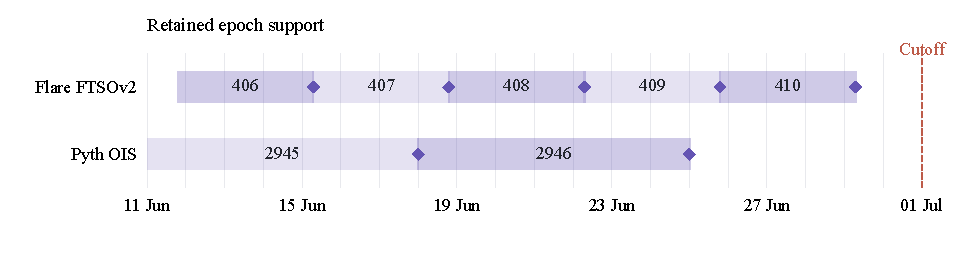
\includegraphics[width=\linewidth]{figures/temporal_epoch_support.pdf}
\caption{Native epochs near the cutoff. Flare and Pyth bars span three and a half and seven days, respectively; diamonds mark epoch-end labels against a daily grid. Labels denote observation intervals, not payments.}
\label{fig:temporal_support}
\end{figure}

\FloatBarrier
\subsection{Temporal availability and coverage}

Timestamp availability is the proportion of retained observations with a valid clock. Historical coverage additionally requires evidence about the period in which a mechanism was active and the intervals successfully collected. A sequence with timestamps on every row can therefore still contain acquisition gaps. Coverage remains unspecified when the underlying observation period cannot be established.

\begin{table}[!htbp]
\centering\tabstyle
\caption{Timestamp availability within retained populations after exact block matching. The Chainlink subset covers staking, withdrawals, reward payments, reward finalization and forfeiture distributions.}
\label{tab:temporal_recovery}
\begin{tabularx}{\linewidth}{@{}Y r Y@{}}
\toprule\tablehead
Observation population & Available & Remaining limitation \\
\midrule
UMA DVM voter accruals & 10.9\% & Execution time is unavailable for unmatched blocks. \\
Chainlink native staking logs & 6.0\% & Retained block references cover only part of the log history. \\
Chainlink analytical subset & 5.0\% & Temporal analysis remains restricted to the dated observations. \\
\bottomrule
\end{tabularx}
\end{table}


Native and UTC timestamps and record selections agree within the tested windows. Subsecond values and native order are preserved, and epoch duration and membership checks support the interval representation. These tests assess processing consistency without establishing clock accuracy or continuous acquisition.


Temporal annotations and the original common representation are separately versioned. Analyses should use a consistent representation and restrict comparisons to compatible observation periods. Daily economic measures further require defined participant roles, assets, economic stages and exposure. Epoch totals should remain attached to their support intervals unless the data justify a more detailed temporal allocation.

\FloatBarrier
\section{Product organization and metadata}
\label{app:products}

The ten logical products group observations by mechanism or reuse task. They do not denote ten physical files or ten independent samples. Native and harmonized representations may describe the same event, and the two derived products draw on the protocol branches. The catalogue therefore records the product membership of each table together with its row unit, source relationship and version.

\begin{table}[!htbp]
\centering\tabstyle
\caption{Ten logical data products and their principal observation units.}
\label{tab:logical_products}
\begin{tabularx}{\linewidth}{@{}L{.19\linewidth}Y Y@{}}
\toprule Product & Principal units & Main relationships \\ \midrule
UMA & Request, vote, voter accrual and stake event & Polygon request--Ethereum adjudication; settlement--transfer \\
Chainlink & Feed update, service interval and staking event & Staking or reward event--LINK movement \\
Tellor & Report, aggregate, dispute and payment & Report--dispute; tip funding--withdrawal \\
Flare FTSOv2 & Provider--epoch, entitlement and claim & Epoch policy--registration; entitlement--claim evidence \\
Pyth & Instruction, reward transfer and publisher--epoch & OIS instruction--custody transfer; historical epoch state \\
Chronicle & Update, challenge and challenge reward & Registered implementation--event; challenge--payment \\
RedStone Push & Adapter/feed update & Registered delivery contract--update \\
DIA & Stake action and withdrawal position & Position--principal and reward components \\
UMA prediction & One eligible request & Proposal-time feature--availability record--resolution label \\
Daily measurements & Date--branch--role--asset--stage--measure & Native eligible population--daily aggregate; epoch companions separate \\
\bottomrule
\end{tabularx}
\end{table}

Field dictionaries specify types, units, economic stage, source keys, missingness and calculation rules. Raw monetary amounts remain integer-valued strings, while UTC clocks distinguish event time from reference time, deadlines, epochs and snapshots. Croissant recordsets describe physical tables and link them to their logical product; the product count is consequently different from the recordset count. The dataset card, table catalogue and tutorial use the same product identifiers.

\FloatBarrier
\section{Daily measurement definitions}
\label{app:daily}

\subsection{Feasibility and coverage}

Feasibility is assessed for each branch and measurement family before aggregation. A derivable quantity is supported within a stated retained population; this designation does not imply continuous acquisition or applicability to every service offered by the protocol. A quantity requiring additional acquisition has a plausible source or linkage requirement. Inapplicable quantities do not describe the sampled unit, whereas unknown quantities lack sufficient evidence to resolve their status. Figure~\ref{fig:feasibility} summarizes selected families; the accompanying matrix includes the full definitions and qualifications.
\begin{figure}[!htbp]
\centering
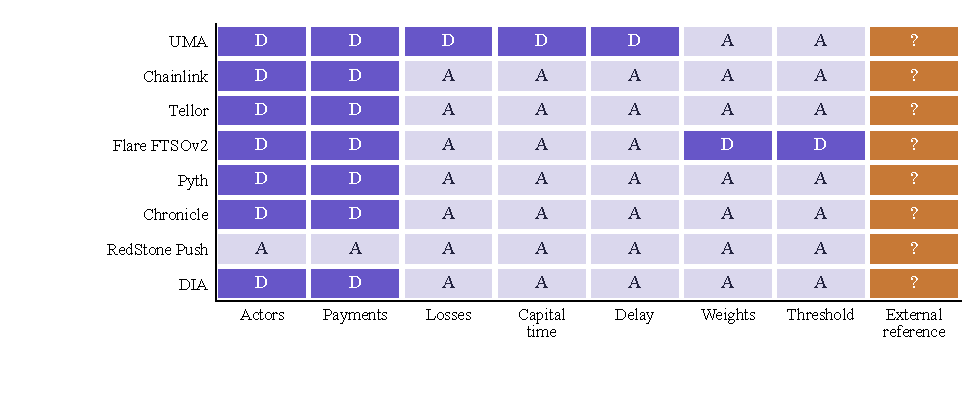
\includegraphics[width=0.99\linewidth]{figures/feasibility_gallery.pdf}
\caption{Measurement feasibility by branch. D: derivable in the retained population; A: additional acquisition or linkage needed; dash: inapplicable; question mark: unresolved. Flare weights and thresholds retain epoch support. RedStone Push covers delivery contracts; publisher participation and AVS economics require separate evidence. }
\label{fig:feasibility}
\end{figure}

\subsection{Aggregation and denominators}

For an eligible event population $\mathcal E_g$ with grouping key $g$, a daily amount is
\begin{equation}
 A_{dg}=\sum_{i\in\mathcal E_g:\,t_i\in[d,d+1)}a_i .
\end{equation}
The grouping key retains branch, implementation, actor role, asset and stage. Integer amounts are summed before decimal conversion. Eligible retained events define the denominator without establishing complete acquisition. Untimed observations cannot enter daily groups and remain in the missingness accounting.

Participation counts distinct observed addresses within a specified role. Delivery-contract activity in RedStone is recorded as contract activity, and Flare reward owners are distinguished from registered providers. Reward inequality uses positive observed recipient totals within the same day, asset and stage. The top-decile share includes the largest $\lceil0.1n\rceil$ recipient totals. A recipient with no recorded payment is outside that recipient population; its absence is not a verified zero reward.

UMA completion delay is measured from the request event to the settlement event and grouped by settlement day. Its denominator consists of completed, flow-reconciled requests. A completion fraction would additionally require a defined obligation and a comparable risk set, so it is not inferred by dividing daily settlements by daily requests. Escrow exposure is computed from the running balance implied by the request's token movements. A request is included only when its lifecycle transactions map unambiguously to that request, all included transfers are timed, balances remain nonnegative and the closing balance is zero. With balance $b_{ik}$ held between successive transfer times $t_{ik}$ and $t_{i,k+1}$, daily exposure is
\begin{equation}
 K_{di}=\sum_k b_{ik}\,\bigl|[t_{ik},t_{i,k+1})\cap[d,d+1)\bigr| .
\end{equation}
The stored quantity uses raw token-seconds; conversion to token-hours divides by the asset precision and 3,600. Fees cease contributing when they leave escrow, while funded rewards contribute for as long as they remain held. The resulting measure describes observed contract balances for the eligible closed-request cohort. It does not establish participant wealth, total protocol collateral or the amount subject to slashing.

\subsection{Historical signing policies}

Flare epoch artifacts record signers, integer weights, a threshold and the starting voting round, matched to retained voter registrations. Normalized weights $w_i$ give concentration $H=\sum_i w_i^2$ and effective address count $1/H$. The table reports the fewest largest-weight addresses needed to reach or exceed the threshold under weak and strict conventions. An operative security threshold requires historical contract and runtime evidence. These address-level measures do not identify owners, independent organizations or attack feasibility.

Entitlements, signing weights and deposited capital retain different units and roles. Epoch values keep their support intervals; uniform daily allocation does not turn reward factors into payments. Signatures and aggregate agreement do not independently measure price accuracy.

\subsection{Temporal sensitivity and lifecycle follow-up}

Weekly aggregation preserves daily event counts and integer amounts within each typed group. A separate comparison restricts observations to the intersection of the branches' retained calendar envelopes. This restriction aligns the outer dates but cannot establish continuous coverage within them. Estimates requiring verified complete intervals therefore remain unavailable. For epoch entitlements, an allocation comparison contrasts the epoch-end label with proportional overlap across UTC days. These are alternative representations of the same entitlement; neither is included among observed daily payments.

UMA follow-up retains settled and unresolved requests until settlement or the common cutoff. Figure~\ref{fig:uma_followup} shows completed-request delays and unresolved shares by request year. Delays are conditional on settlement, and cohorts have unequal follow-up. Neither panel estimates protocol-wide timely-resolution probabilities.
\begin{figure}[!htbp]
\centering
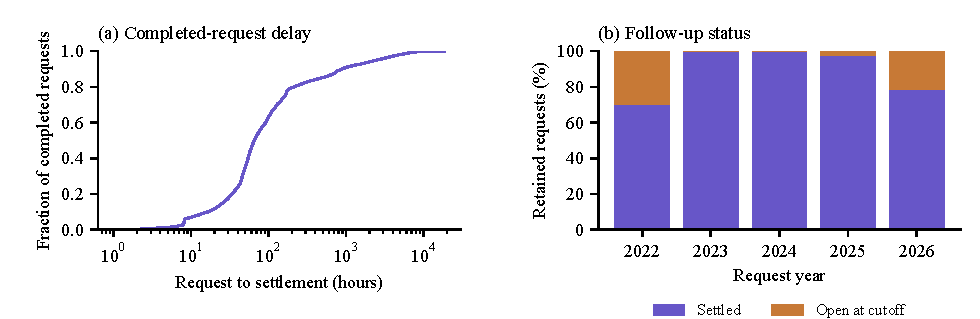
\includegraphics[width=0.99\linewidth]{figures/uma_followup.pdf}
\caption{UMA request follow-up. (a) Empirical cumulative distribution of elapsed request-event to settlement time among completed requests. (b) Settlement status at the common cutoff, grouped by the year of the request event. Requests still open at the cutoff are right-censored; an unobserved later settlement is not classified as failure.}
\label{fig:uma_followup}
\end{figure}

\FloatBarrier
\section{Semantic rules and assistance disclosure}
\label{app:semantics}

The correction ledger links changed fields to native objects, historical rules and prior interpretations. UMA challenge status requires a dispute; settlement requires completion and the relevant token flow. Winner payouts separate principal from the unburned losing bond. Tellor SUPPORT accepts the challenge; an AGAINST outcome does not imply reporter loss merely because stake previously entered escrow.

VotingV2 requires a further distinction between request-level accrual and application to stake. A signed accrual records an adjustment associated with a voting request. The later application event concerns the net change actually applied to a stake position. The ledger retains the accrued amount and leaves a request-level applied loss unknown when application evidence is not matched. Adding the accrual to a subsequent net application would count stages of the same accounting process twice.

Historical binding is assessed separately from arithmetic. Evidence is stronger for VotingV2 than for OOv2 and Tellor. A commit identifies inspected code but does not prove which binary executed at each block. Table~\ref{tab:semantic_repair} reports corrections only for the tested populations.

Codex assisted with source inspection, processing code, manuscript editing and figures; the assistance record documents its contributions and available model information. Automated checks assess consistency and reconstruction, while economic interpretation remains limited by the historical source evidence.

\FloatBarrier
\section{UMA task definition and feature dictionary}
\label{app:prediction}

The task contains 810 retrospectively eligible requests, of which 466 resolve to a value different from the proposal and 344 retain the proposed value. A changed value is an institutional adjudication label. The cohort is restricted to challenged, linked and reconciled requests, so these proportions do not estimate the prevalence of incorrect proposals in the full request population.

Excluding early expiration leaves 413 requests with 69 changed proposals; restricting resolutions to binary zero or one leaves 402 requests with 59 changes. These cohorts support sensitivity analysis. The main task keeps native classes because early expiration differs from either binary outcome.
\begin{figure}[!htbp]
\centering
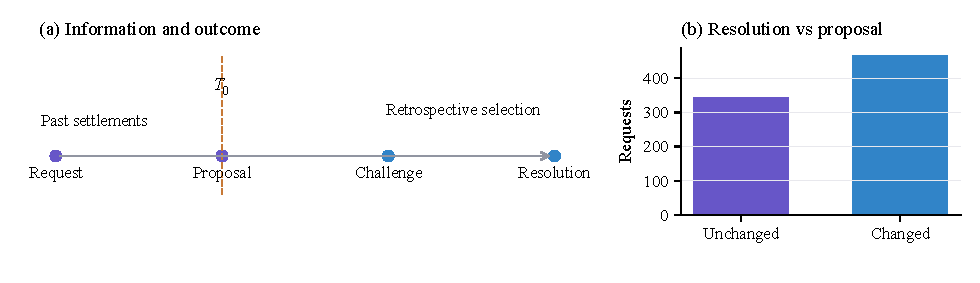
\includegraphics[width=0.99\linewidth]{figures/prediction_task.pdf}
\caption{Information boundary and target of the UMA task. (a) $T_0$ is the proposal event; prior-history features use earlier settled requests. Challenge and resolution determine retrospective eligibility and the outcome. (b) Counts compare the native proposed and resolved integers, retaining special resolution classes.}
\label{fig:prediction_task}
\end{figure}

Let $B$, $F$ and $R$ denote the effective bond, final fee and configured reward in the asset's smallest units. For address $a$ in a specified role, $N_a$ counts retained prior settlements, $D_a$ counts those challenged, and $J_a$ counts those whose challenged proposal was rejected. Prior settlements must precede the proposal in block, transaction and log order. Proposer and requester histories are separate and bounded by the retained records.

\begin{table}[!htbp]
\centering\tabstyle
\caption{Sixteen candidate features. Rates with $N_a=0$ and ratios with $B=0$ are missing. Parameter-derived entries require historical binding before they can be certified as available at the proposal.}
\label{tab:prediction_features}
\begin{tabularx}{\linewidth}{@{}L{.30\linewidth}L{.24\linewidth}Y@{}}
\toprule Feature & Definition or unit & Evidence / missingness \\ \midrule
Bond magnitude & $\log(1+B)$ & Reconstructed effective bond; historical parameter binding. \\
Final-fee magnitude & $\log(1+F)$ & Native fee; missing if absent. \\
Reward magnitude & $\log(1+R)$ & Configured adapter reward; historical binding. \\
Reward--bond ratio & $R/B$ & Same-asset amounts; undefined for zero bond. \\
Liveness & Expiry minus proposal, hours & Proposal event and recorded expiry. \\
Proposal latency & Proposal minus request event, hours & Execution clocks, not request-reference time. \\
Ancillary length & Decoded byte count & Native request payload. \\
Proposer prior count & $N_a$ & Earlier settlements in proposer role. \\
Proposer dispute rate & $D_a/N_a$ & Missing when no prior settlement is retained. \\
Proposer rejection rate & $J_a/N_a$ & Rejected challenged proposals among prior settlements. \\
Requester prior count & $N_a$ & Earlier settlements in requester role. \\
Requester dispute rate & $D_a/N_a$ & Missing when no prior settlement is retained. \\
Requester rejection rate & $J_a/N_a$ & Same-role prior settlement outcomes. \\
Registered adapter & Binary membership & Requester contract registry. \\
Proposed price class & Zero, one, half, early expiry, other & Native proposed integer; no forced binary recoding. \\
Adapter version & Registered implementation class & Historical source binding required. \\
\bottomrule
\end{tabularx}
\end{table}

Feature availability is recorded for each request and feature. Native event fields, reconstructed past histories and parameters requiring historical binding have distinct statuses. Fields used only to establish the eventual label remain outside the feature allowlist. Missing rates are retained as missing values so that subsequent users can choose and document their own preprocessing. Figure~\ref{fig:prediction_features} presents the feature distributions; no predictive model is fitted as part of this data description.
\begin{figure}[!htbp]
\centering
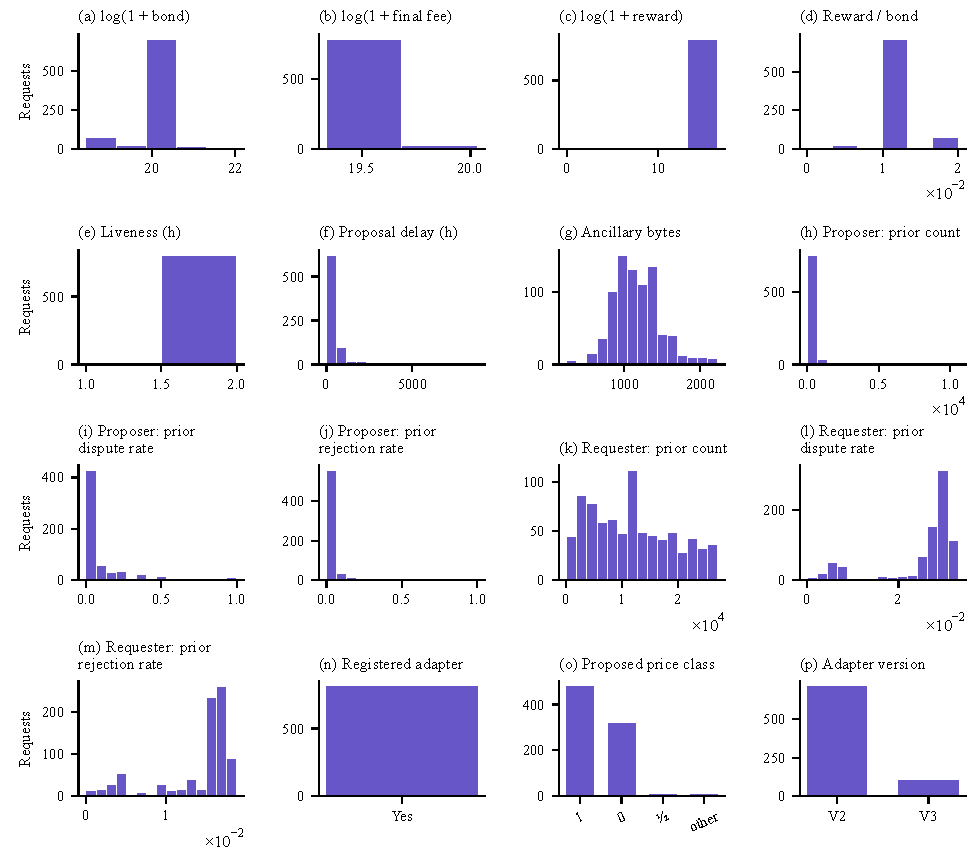
\includegraphics[width=0.99\linewidth]{figures/prediction_features.pdf}
\caption{Distributions of the sixteen task features. Histograms use nonmissing observations on the units in Table~\ref{tab:prediction_features}; categorical panels retain the recorded classes. Prior-history rates exclude requests with no retained earlier settlement in that role. Detailed missingness and availability statuses accompany the task data.}
\label{fig:prediction_features}
\end{figure}

\FloatBarrier
\section{Cross-chain event register}
\label{app:case}

The worked case is a single OOv2 request linked to one VotingV2 request. Table~\ref{tab:case_events} locates the five observed endpoints. Full contract addresses, request identifiers, transaction hashes and receipt evidence accompany the register. A log position is interpreted within its transaction and chain; equal-looking identifiers on different chains are not joined without the registered ancillary-data transformation.

\begin{table}[!htbp]
\centering\tabstyle
\caption{Observed endpoints of the worked UMA dispute. UTC coordinates identify actual case events. Explorer links locate the transactions; retained receipts provide the reproducible evidence.}
\label{tab:case_events}
\begin{tabularx}{\linewidth}{@{}L{.22\linewidth}L{.12\linewidth}L{.27\linewidth}Y L{.12\linewidth}@{}}
\toprule Event & Chain & UTC & Block / log & Evidence \\ \midrule
T1 Request & Polygon & 2024-10-29 20:05:50 & 63645613 / 196 & \href{https://polygonscan.com/tx/0x6fc39485f25f23d42bcb55baf68633b31aa5aa53a881116ecf1382e6a1245ede}{Transaction} \\
T2 Proposal & Polygon & 2024-10-30 03:47:16 & 63658346 / 327 & \href{https://polygonscan.com/tx/0xa9ff6827a32b90f134345bbc646a480787676f481ac651b00088520379b47903}{Transaction} \\
T3 Dispute & Polygon & 2024-10-30 03:49:54 & 63658420 / 397 & \href{https://polygonscan.com/tx/0xa5742b4d0b43dbe96de0e57480fbc11a6aa61c64765395db9f27ae45ae5b2198}{Transaction} \\
T4 DVM resolution & Ethereum & 2024-11-03 00:00:35 & 21103395 / 141 & \href{https://etherscan.io/tx/0xc845c4be3da71936e760b5fb8b70eeb8753a7bc5012c452e7d335166d9b14039}{Transaction} \\
T5 Settlement & Polygon & 2024-11-03 00:22:35 & 63813887 / 104 & \href{https://polygonscan.com/tx/0xe9457425a7a67a5e1bb431a7e3b1f8fe4649fcf04f3bb74376caa15600420310}{Transaction} \\
\\[-1.4ex]\bottomrule
\end{tabularx}
\end{table}

The Polygon request, proposal and dispute are decoded from OOv2 events; Ethereum's resolution is decoded from VotingV2. The Polygon settlement retains the same resolved value. Native request hashing and ancillary-data transformations support the identity match. The five retained transactions do not provide a complete sequence of relay acceptance, processing and return operations, so the interval between dispute and resolution is not attributed solely to voting or solely to transport.

\begin{figure}[!htbp]
\centering
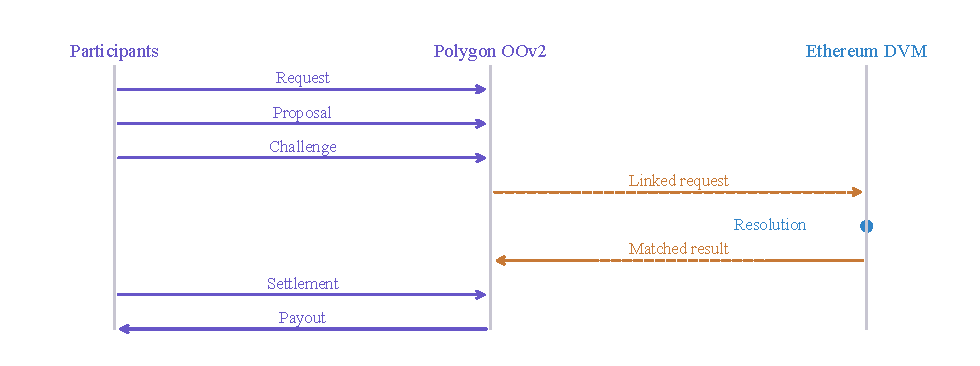
\includegraphics[width=0.99\linewidth]{figures/cross_chain_evidence_links.pdf}
\caption{Evidence links in the worked case. Solid arrows denote observed participant actions or transfers. Dashed arrows connect matched request identities and outcomes across chains; they do not represent an independently reconstructed relay path. Vertical order is schematic. Elapsed times are shown in Figure~\ref{fig:case}.}
\label{fig:cross_chain_links}
\end{figure}

Accounting separates both deposits, the winner's gross payout and the protocol fee. Principal return and gain decompose one payout and must not be added again as transfers. The configured reward is tracked separately. Early expiration retains its native meaning; the proposition lacks independent factual adjudication.

\FloatBarrier
\section{Reconstruction and versioned evidence}
\label{app:reproduction}

Reproducibility is organized around the relationship between retained inputs, deterministic transformations and named outputs. Input fingerprints bind a calculation to the files it used. Source registries identify the interfaces and historical boundaries, while result manifests connect tables and figures to the relevant processing rules. A successful replay establishes consistency for those inputs and transformations.

The tutorial provides one bounded example per branch, checking retained inputs, native units and clocks. Fresh historical queries depend on archive retention and provider behaviour. Retrieving an individual receipt or block does not establish continuous acquisition across the registered interval.

The reproduction record documents commands, environment versions, validation and acquisition limits. Earlier model experiments remain separate from the revised feature definitions. The catalogue and checksums identify this revision's materials and distinguish them from previous public deposits.

\FloatBarrier
\clearpage
\section{Measurement glossary}
\label{app:glossary}

\begin{table}[!htbp]
\centering\tabstyle
\caption{Terms used to distinguish protocol activity, economic states and evidence.}
\begin{tabularx}{\linewidth}{@{}L{.25\linewidth}Y@{}}
\toprule Term & Meaning \\ \midrule
Branch & Registered mechanism and implementation scope, with specified chain roles. \\
Observation unit & Native object counted or measured, such as a request, claim or provider--epoch. \\
Configured incentive & A rule or parameter describing a potential reward or penalty. \\
Accrual & An accounting adjustment associated with an activity, before separate application or payment evidence. \\
Entitlement & A recorded claim to an amount under the applicable eligibility rules. \\
Realized payment & A qualifying transfer or execution record under a stated branch-specific rule. \\
Applied loss & A supported reduction or forfeiture; not inferred from every negative accrual. \\
Principal return & Recovery of posted capital, distinct from income. \\
Escrow exposure & Observed token balance integrated over time, including funded rewards while held and retaining the eligible request population. \\
Policy weight & A mechanism-specific influence measure; not automatically collateral or organizational independence. \\
Coverage state & Evidence about what was observable and collected for a particular population or interval. \\
Protocol adjudication & An institutional resolution; external truth requires independent evidence. \\
\bottomrule
\end{tabularx}
\end{table}

\FloatBarrier
\end{document}
